\documentclass[a4paper,12pt]{report}
\usepackage{setspace}
\usepackage{relsize}
\usepackage{graphicx}
\usepackage{tikz}
\usetikzlibrary{trees}
\usepackage{float}
\usepackage{commath}
\usepackage{geometry}
\usepackage{listings}
\usepackage[toc,page]{appendix}
\usepackage[toc,acronym]{glossaries}

% Set the overall layout of the tree
\tikzstyle{level 1}=[level distance=3.5cm, sibling distance=3.5cm]
\tikzstyle{level 2}=[level distance=3.5cm, sibling distance=2cm]

% Define styles for bags and leafs
\tikzstyle{bag} = [text width=4em, text centered]
\tikzstyle{end} = [circle, minimum width=3pt,fill, inner sep=0pt]

\definecolor{mygreen}{rgb}{0,0.6,0}
\definecolor{mygray}{rgb}{0.5,0.5,0.5}
\definecolor{mymauve}{rgb}{0.58,0,0.82}

\lstset{
  backgroundcolor=\color{white},   % choose the background color
  basicstyle=\footnotesize,        % size of fonts used for the code
  breaklines=true,                 % automatic line breaking only at whitespace
  captionpos=b,                    % sets the caption-position to bottom
  commentstyle=\color{mygreen},    % comment style
  escapeinside={\%*}{*)},          % if you want to add LaTeX within your code
  keywordstyle=\color{blue},       % keyword style
  stringstyle=\color{mymauve},     % string literal style
  numbers=left,					   % add line numbering
  numberstyle=\footnotesize,		   % set numbering styel
  stepnumber=1,					   % set numbering increment
  language=Java					   % set langauges
}

\newcommand{\nocontentsline}[3]{}
\newcommand{\tocless}[2]{\bgroup\let\addcontentsline=\nocontentsline#1{#2}\egroup}

\makeglossaries

\newglossaryentry{congstats}
{
        name=CONGSTATS,
        description={is a software product, part of a development contract in which the thesis was conceptualized. Its goal is to supply a statistical analysis tool for engineers examine traffic data}
}
\newglossaryentry{evaltool}
{
        name=evaluation tool,
        description={is part of the CONGSTATS service and was adapted and expanded for the usage in this thesis. It handles the analysis of processed \acrshort{fcd} data, congestion detection, incident matching and exports the analysis data}
}
\newglossaryentry{speedmatrix}
{
        name=Speed Matrix,
        description={is the data format of the processed \acrshort{fcd} data is a two-dimensional integer matrix representing a non-Euclidean time to road link space with the corresponding mean cell speed as value. The time dimension referrers to the 3-minute time increment of the day and the space dimension to the road link of the covered route of the speed matrix.}
}
\newglossaryentry{jam}
{
        name=congestion,
        plural=jams,
        description={ \textbf{or jam} is the spatial and timely accumulations of traffic participants, which leads to a reduction of travel speed and therefore reduction of traffic throughput. Because the plural of the noun congestion is not clearly recognizable, in the context of multiple congestion, the term \glspl{jam} will be used. A more detailed definition of a congestion can be found in chapter \ref{definition_congestion}}
}
	

\newacronym{fcd}{FCD}{Floating Car Data}
\newacronym{fco}{FCO}{Floating Car Observer}
\newacronym{csv}{CSV}{Comma-seperated Values}
\newacronym{gsm}{GSM}{Global System for Mobile Communications}
\newacronym{umts}{UMTS}{Universal Mobile Telecommunications System}
\newacronym{lte}{LTE}{Long Term Evolution}
\newacronym{arbis}{ArbIS}{Arbeitstellenintegrationsystem}
\newacronym{ari}{ARI}{Autofahrer Rundfunk Information}
\newacronym{baysis}{BAYSIS}{Bayrische Straßeninformationssystem}
\newacronym{fpd}{FPD}{Floating Phone Data}
\newacronym{rtti}{RTTI}{Real Time Traffic Information}
\newacronym{tmc}{TMC}{Traffic Messaging Channel}
\newacronym{xfcd}{XFCD}{Extended Floating Car Data}
\newacronym{zvm}{ZVM}{Zentralstelle Verkehrsmanagement}
\newacronym{gps}{GPS}{Global Postioning System}

\onehalfspacing
\begin{document}
% Title page goes first
\title{MASTER'S THESIS\\
[1cm]
\smaller Analysis of correlation between traffic data depended congestion detection and incident causalities}
\author{
B. Sc. Jakob Erpf\\ 
[1cm]
\small Mentoring:\\ 
\small M. Eng. Barbara Karl (TUM)\\ 
\small Dr. - Ing. Matthias Spangler (TUM)\\ 
\small Dipl. - Ing. Stefan Gürtler (S\&W)\\
\small Dipl. - Ing. Johannes Grötsch (LBD)
}
\date{\today}
\maketitle
% Empty page for layout purpose
\clearpage
% Topic description is mandatory
\renewcommand\abstractname{Topic}
\abstract{}
Date of Issue: 2020-05-04\newline
Date of Submission:	2020-12-11\newline
\newline
\par The \gls{congstats} service is a statistical analysis tool, developed by the Munich office of SCHLOTHAUER \& WAUER GmbH and the thesis writer for the road administration of north and south Bavaria, to request and analyze traffic data. The traffic data used in this service is based on \acrfull{fcd}, provided by the Bavarian road administration. The aim of the service is to provide statistical monitoring and report functionalities on the traffic situation on freeway and state street network, to identify congestion-prone areas.
\par An interesting aspect of this congestion analysis is the correlation of congestion events and incidents. What are the circumstances leading to congestion in cause of an incident? What are the dependencies on an occurred incident, for example roadworks or accident? The knowledge on the impact of roadworks on the traffic flow or which accidents lead to traffic capacity reductions could improve traffic management and incident response actions. The question of how the congestions rep-resented by the \acrshort{fcd} correlate with actual traffic incidents and their probably causalities, will be evaluated in this thesis. 
\par To answer this research question, the writer will be provided with a dataset of traffic data from the CONGSTATS service, which contains congestion and incident data, as well as the service itself. The \acrfull{zvm} provides the incident’s reports, which hold statistics on the traffic incident situation and detailed reports for the specific incidents.
\par These two datasets then can be analyzed for possible correlations between the detected congestions in the \acrshort{fcd} model and the reported incidents from the \acrshort{zvm}. The scope of the thesis consists of the following tasks:
\begin{itemize}
  \item review of the available data and information
  \item definition data characteristics and indicators
  \item definition and implementation of a methodology for analyzing the correlation between congestion and incident
  \item analysis of the provided datasets
  \item interpretation of the results
\end{itemize}
\par The student will present intermediate results to the mentors 
		(Barbara Karl, M.Eng.: TUM-VT; 
		Dr.-Ing. Matthias Spangler: TUM-VT; 
		Dipl.-Ing. Stefan Gürtler: Schlothauer \& Wauer; 
		Dipl.-Ing. (FH) Johannes Grötsch: ZVM) 
	in the fifth, tenth, 15th and 20th week.
\par The student must hold a 20-minute presentation with a subsequent discussion at the most two months after the submission of the thesis. The presentation will be considered in the final grade in cases where the thesis itself cannot be clearly evaluated.
% Germany abstract
\renewcommand\abstractname{Kurzfassung}
\abstract{Deutsche Fassung.}
% Englisch abstract
\renewcommand\abstractname{Abstract}
\abstract{Current navigation systems often use accumulation strategies to estimate travel time with considering time delays through congestions, which are based on analyzing the history of the time delays on the considered street network. This approach can be disturbed through un-common events creating short time blockages or be bias through regular accruing and long-er-term traffic volume reductions. This thesis evaluates a new idea of predicting time delays and accident probability through analyzing the correlation of congestions and incidents which are placed in the timely and spatial vicinity of each other. To evaluate this, three real world datasets from the year 2019 will be considered. After an initial data scientific approach to analyzing a derivative of a floating car dataset for congestions and locating spatial and timely adjacent incidents from the Bavarian street information systems, the thesis will evaluate if and how incidents and congestions are correlated with each other. To further give an idea of how such statistical data could be used, the thesis will elaborate on the possibility and plausibility of using correlation statistics for congestion and/or incident prediction.}
% Disclaimers
\renewcommand\abstractname{Preliminary information and disclaimers}
\abstract{
Datennutzungserklärung\newline

During the elaboration of the evaluation tool, which was not only developed for the thesis, the mentioned capabilities do not represent the final functional range of the software. Since the tool was still in early development most of the information about the functionalities and capabilities are already outdated when writing the thesis}

%\setcounter{secnumdepth}{3}
%\setcounter{tocdepth}{3}\
\tableofcontents
\thispagestyle{empty}

\chapter{Introduction}
\setcounter{page}{1}
Traffic \glspl{jam} are a known problem to everyone, ever attempting to kickstart the summer season with a car trip on the first day of a holiday. They also impact the regular travel of commuters urban and suburban areas with blocking bottlenecks and reducing travel speeds, resulting in more than 500.000 hours in time losses \cite{ADAC2019} per year. They lead to unreliable travel times, inefficient usage of resources, and an increase in emissions, like pollutants or noise. Another common effect it a decrease in road safety, because of high driver tempers or inattentive mind, which can result in higher accident counts \cite{Sun2016}. They also induce enormous social costs due to the time losses in \glspl{jam}, ranging in the higher billions per year. \cite{RetallackOstendorf2019,BardtFritsch2014}

It is therefore essential to reduce the risk of \glspl{jam}, as well as accidents, with an increased understanding of the causes of traffic accidents, particularly \glspl{jam}, to maintain fluent traffic flow. Additionally increased knowledge of the formation effects of roadworks leading to jams could enable tailored management of high traffic demands in reduced traffic volume areas. All this would go towards reducing the economic, environmental, and social costs associated with accidents, roadworks or \glspl{jam} and could be achieved through the facilitation of improved traffic infrastructure design and traffic management. Part of this advanced traffic management could be the development of a traffic prediction systems to reduce accidents, with the potential to identify hazardous conditions in real-time, allowing according to actions to be taken to avoid consecutive events. \cite{RetallackOstendorf2019} 

\bigskip

This thesis takes another attempt to improve \gls{jam} and incident prediction by evaluating the statistical relation of \glspl{jam} and incidents to predict the chance of a consecutive event. These consecutive events can have the form of \gls{jam}, as well as an incident since dependent on the severity of the incident a \gls{jam}, can be provoked or \glspl{jam} can facilitate accidents due to the change of traffic flow. Another scenario is construction sites and maintenance which can also lead to both \glspl{jam} and accidents, because of the reduction of traffic volume, changes in road guidance, or other modifications to the normal traffic situation.  


The ability to predict \glspl{jam} through the characteristic of an accident could help to improve traffic controlling and therefore help to still ensure fluent traffic for lower emissions and static traffic safety. The same can be expected for the prediction of an accident through the characteristic of jams and tailoring traffic controlling actions to prevent the above mentioned. Although the scope of the thesis does not cover the specifics on a complete production system for \gls{jam} and accident detection, prediction and response, it will take the concept of such a system and focus the possibility of predicting such events, which then would make the development of such a system possible. 
\par A system capable of the described mentioned functionalities would likely consist of the following processing components.

\begin{itemize}
  \item Data acquisition for congestion and incident detection
  \item Data analysis for the probability of consecutive events
  \item Traffic management and controlling response channel
\end{itemize}

\par The first component, in charge of detecting \glspl{jam} as well as incident, requires input data like speed, volume, occupancy to represent the traffic situation and incident reports to define incident characteristics. The next component would then analyze the resulting dataset to find characteristic features of the congestions and incident, which will be determined in this thesis. In the case the analysis of the characteristic shows a quite possible and imminent event it would trigger the last component to initiate appropriate controlling actions and prepare incident responses.\newline
\par In the following chapters of this introduction section, the reader will be introduced to the concepts and systems used to cover the input and output requirements in this thesis.

\section{Continuous Floating Data}

\par To detect \glspl{jam}, continuous data about the speed at each point of time on the road is necessary. This kind of information can be collected through a variety of different systems, to represent a real-time or at least current picture of the traffic situation. The current street net-work of Bavaria still heavily depends on stationary sensors, to assess the traffic situation. This includes inductive loops, infrared or radar detectors, which can provide traffic indicators like volume, speed, time gaps, jams, density and many others. The data collected with just stationary sensors can only describe the traffic trends restricted to its location and coverage, which requires complex simulations and modeling to aggregate data for the missing areas where there is no sufficient coverage. Adding to this is the fluctuating result set quality which depends on the input data and simulation model quality. In Germany especially highways are equipped with stationary sensor, but the lower index streets network is only covered by a fragmented net of detectors with distances of up to 100km between detectors \cite{INDRIX2015}. Fortunately, nowadays cars as well as drivers and riders are equipped with technology that allows real time tracking and area-wide data collection. Cars can gather information from the build in sensors as well as an on-board GPS and mobile devices from drivers and riders can also be used to collect location and movement data. \cite{Randelhoff2016}

\par \acrfull{fcd} is continuously collected during the usage of a car by the on-board GPS and represents the individual movements. Typical this incorporates the coordinates, timestamp, road section, course and routing data points. These are regularly sent to a central FCD unit/service via mobile radio communication (\acrshort{gsm}-, \acrshort{umts}- or \acrshort{lte}-based), to be aggregated and combined with stationary data to an area wide picture of the traffic situation. In this form they can be used for traffic analysis and management. \cite{Randelhoff2016,LAPID2020}

\par A derivative of \acrshort{fcd} is \acrfull{xfcd}, developed by BMW. It expands the collection of datapoint of an \acrshort{fcd} with data from the vehicle sensors and systems, like breaks, rain sensors, driver assistance systems and more. These data points add a number of possible analytic opportunities to generate a more precise and details traffic picture. \cite{LAPID2020}

\par In contrast to \acrshort{fcd}, \acrlong{fpd} does not need an on-board GPS or car systems to create movement data but assumes that driver’s and rider’s mobile devices will register and deregister at the radio tower along the road. \acrshort{fpd} uses this registration information to determine the radio cell the phone is currently in, how long is stayed in that cell and tracks the devices when switching to another cell or tower. It is therefore able to collect a much larger quantity of datasets but lacks the accuracy of \acrshort{fcd} which transmit the GPS location of the car itself. That been said, on roads with a high coverage of radio tower like in urban areas or on highways, \acrshort{fpd} is able to generate a comparable accuracy. Mobile service providers collect this anonymized \acrshort{fpd} and forward them to a traffic management unit, which can analyze the date for disturbances and give feedback through the traffic information channels. \cite{Randelhoff2016,LAPID2020}

\par Another type of floating data type is \acrfull{fco}. \acrshort{fco} does not only collect its own \acrshort{fcd} but also data about its surrounding with the build-in sensors. This includes the automatic recognition of cross or opposite traffic, traffic volume or relative speeds to other cars. This additional data not only add detail, but also allows for correctional fusion algorithms to eliminate uncertainties or errors in the pure \acrshort{fcd} data. \cite{Randelhoff2016}

\section{Street Information Systems}

\par Besides of having a real-time or current picture of the traffic situation, the concept of the the-sis also needs information about current disturbances or possible triggers of disturbances. For disturbances in the form of accidents the \acrfull{baysis}, a public available information system from the Bavarian street administration, will be used. The systems task is the acquisition, collection and analysis of street network related information, which contains infrastructure inventory and condition, traffic volumes and other key values, as well as an accident register with detailed reports. An export of this accident register with detailed report is provided by the \acrshort{zvm} for this thesis.

\par Another type of disturbance to consider are roadworks, for which an export from the \acrfull{arbis}, a software tool and database used by the Bavarian infra-structure ministry, will be consulted. The system is used to collect and archive all current, planned and passed roadwork and maintenance projects on the Bavarian state street net-work. Thought the coordinated and traffic safety depended planning of road maintenance with the collected information from \acrshort{arbis}, an effective, economic and safe execution of roadworks can be achieved. Furthermore \acrshort{arbis} can provide detailed report exports about current projects to the Bavarian traffic information office and traffic information channels. \cite{trafficon2017}

\section{Traffic Status Information}

\par To deliver information from traffic management system to the traffic participants traffic messaging channels can be used. Two examples are \acrfull{rtti} and \acrfull{tmc}.

\par The \acrfull{tmc} is a messenger system for congestions and other traffic incidents. The public available service published current congestion notifications in navigation system and in announcements in the local radio channels. To define where an incident is located, in the scope of the \acrshort{tmc} the road network is split into \acrshort{tmc} sections. These sections typical start and end with road linkups. The \acrshort{tmc} obtains data from the police and re-ports from traffic participants. \cite{LAPID2020}

\par Another traffic information source is the \acrfull{rtti}. \acrshort{rtti} supplies traffic participants with information about current events or suggested diversions and can be compared to the \acrfull{ari}, with one big difference. Through a “Geocast”, which is expansion of a multicast with a geolocation, the spatial precision of the \acrshort{rtti} is superior to the \acrshort{tmc}. This geolocation can be either a geometrical address like a GSM84 coordinate or a symbolic address like an area alias. \cite{LAPID2020,HindenDeering2006,ImielinskiNavas1996} \newline

% TODO more infos and literature to TMC / Geocasts
%https://ec.europa.eu/transport/themes/its/road/action_plan/traffic-information_en
%https://www.itwissen.info/RTTI-realtime-traffic-information.html
%https://ieeexplore.ieee.org/document/861224

\par In the scope of this thesis only a selection of these introduced data collection systems will be further relevant in this thesis. 
\begin{itemize}
  \item \acrshort{fcd} for the congestion detection
  \item \acrshort{baysis} and \acrshort{arbis} as incident data providers
  \item \acrshort{rtti} as conceptional feedback channel
\end{itemize}

\chapter{Definitions}
	This chapter defines the key terms which will be referenced to during the thesis.
\section{Incident}
		Incidents in the scope of this thesis, an incident can be accidents, as well as ongoing roadwork or maintenance on the Bavarian street network. These are also the events, which the concept of the thesis tries to predict through the analysis of the correlation of said incidents to jams.
	\subsubsection{Accident}
		An accident is an unexpected and unintentional traffic event, that typical results in damages, injuries and reduction of traffic volumes. These events can be triggered a number of different reasons, where in this thesis we a mostly interested in the trigger of slow, congested traffic or roadworks.
	\subsubsection{Roadwork}
		As roadwork classify all static and moving construction sites, as well as temporary blockages or disturbance due to snow clearing, road maintenance and alike. 
	
\section{Congestion}
\label{definition_congestion}

\paragraph{Naming} The noun congestion does not have clear plural, which is why in the case of multiple congestion, the term jams will be used. These two terms are seen as interchangeable for their reference to a single or multiple congestion events.

\bigskip

Jams or a single congestion in most colloquial terms are spatial and timely accumulations of traffic participants, which leads to a reduction of travel speed and therefore reduction of traffic throughput. But there is no unified definition when this reduction of speed or volume can be actually classified as a congestion. As an example the ADAC classifies highway traffic moving with mean speed lower than 20 km/h as jammed \cite{ADAC2019}. In Switzerland the ministry for streets has a more severe definition with a mean speed under 10 km/h \cite{ASTRA2020}. The Germany or Bavarian ministry for streets does not have an official definition at the time of writing, which makes it necessary to form our own definition of jams and speed thresholds, for the scope of this thesis. Because we have a good representation of the speeds occurring in jams from the FCD date, introduced in chapter 1.1, we can use this information to tailor a definition to our needs. The Figure \ref{img:speedMatrixPlot_singleCluster} on page \pageref{img:speedMatrixPlot_singleCluster} shows a section of a random speed matrix plot from the FCD dataset, containing a scattered congestion cluster. The horizontal and vertical extend represents the spatial and temporal location of each cell. The color of the cell indicated the mean absolute speed recorded in the time frame and on the link of the cell (detailed gradient is shown in the legend of \ref{img:speedMatrixPlot_singleCluster}). The visual representation show that a congestion mostly contains speed of less than 30 km/h, shown in \textit{dark red}. A closer look on the cluster in the top left reveals that speed around 40-50 km/h, shown in \textit{lighter red} tones, may be also considered as jammed, to incorporate the complete congestion area. Speeds above 50 km/h, starting with the \textit{orange/yellow} categories, should not be included in the definition, because it would classify regular speed limits, represented by the broad vertical \textit{orange/yellow} stripe, as jammed traffic. This makes a speed threshold of 40 km/h fitting for detecting congestion clusters in the scope of this thesis.

\begin{figure}[h]
	\centering
	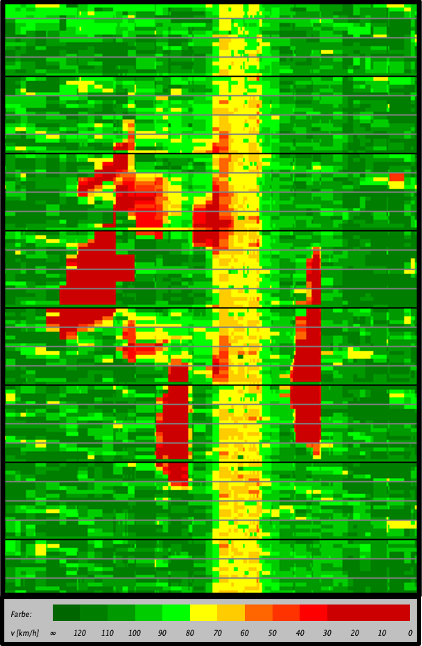
\includegraphics[scale=0.8]{./assets/SpeedMatrixPlot_single}
	\caption{Speed matrix plots of raw FCD data, showing a scattered cluster}
	\label{img:speedMatrixPlot_singleCluster}
\end{figure}

\bigskip

More Infos about what characteristics do congestions have? Causes, Effects and Indicators...

%https://www.astra.admin.ch/astra/de/home/themen/nationalstrassen/verkehrsfluss-stauaufkommen/definitionen.html
%https://www.sciencedirect.com/topics/social-sciences/traffic-congestion
%https://ops.fhwa.dot.gov/congestion_report/chapter2.htm
%https://www.zukunft-mobilitaet.net/3344/analyse/wie-entstehen-staus-phantomstau/
%https://diglib.tugraz.at/download.php?id=576a764ebc982&location=browse

\bigskip
\bigskip
\bigskip

\chapter{Correlation}
\label{definition_correlation}
Correlation is an analysis procedure that measures the correlation coefficient, which represents the degree of linear, bivariant, monotonic or other kind of relation, which could also be described as the degree of association between two variables \cite{HerzSchlicherSiegener1992}. In most statistics the following common types of can be found: Pearson's $r$, Kendall's $\tau$, Spearman  $\rho$ or the Point-Biserial correlation \cite{Ramzai2020,SPSS2020a,SPSS2020b}. Besides off these, there are many more correlation coefficients which varying in they applicability and interpretability. Depending on which type of data variables are to be analyzed, it it necessary to choose an applicable correlation coefficient. In this thesis the type of data variable to be examined is the most restricting feature for choosing a suitable correlation coefficient and therefore the primary criterion. 

\section{Variable Types}
\label{correlation_variable_types}
Data variables can be grouped into continuous and categorical, depending what kind of observation they describe. Variables are considered to be continuous, also know as quantitative, when relating to measurements like speed, distance or age, which can take on an unlimited number of values between the lowest and highest points of measurement \cite{McCue2007}. These continuous variables can be separated into two subsets. 

\begin{itemize}
	\item \textbf{Interval} variables can be measured along a continuum and have a numerical value. \cite{Laerd2020}
    \item \textbf{Ratio} variables are interval variables, with the added condition that the values is zero if there is no measurement for this value. \cite{Laerd2020}
\end{itemize}

Categorical variables on the other hand are limited in the number of values, referring to a category, rank or choice, like a vehicle type or Yes/No answers. These categorical variables can be separated into three subsets.

\begin{itemize}
	\item \textbf{Nominal} variables have two or more categories, but with no intrinsic order. \cite{Laerd2020}
	\item \textbf{Dichotomous} are nominal variables which have only two categories or levels. \cite{Laerd2020}
    \item \textbf{Ordinal} are nominal variables that have two or more categories and are ordered or ranked. \cite{Laerd2020}
\end{itemize}

The datasets to be examined in this thesis include continuous variables of the type interval, as well as all three types of categorical variables (see \ref{dataset_baysis} and \ref{dataset_arbis}).

\section{Coefficient Types}
\label{correlation_coefficient_types}
The provided (see \ref{dataset_baysis} and \ref{dataset_arbis}) and generated (see \ref{methodology_data_generation}) datasets includes continuos, as well as categorical variables, describing interval, nominal, dichotomous and ordinal characteristics. That makes it necessary to choose the appropriate correlation coefficient suited for the apparent variables. In the following a number of coefficients, prominent in current statistic literature will be evaluated.

\subsubsection{Continuous - Continuous}
Pearson $r$ describes the linear correlation of continuous, non-ranked variables. It does not assume normality or a normal distributed sample set and is therefore suitable for the examination of continuous-continuous variable relations, where we can assume finite size of variance and covariance \cite{BenestyChenHuang2009, Sulthan2018}. 

In the case of rank ordered continuous variables the commonly used Spearman's $\rho$ can be applied, but should be replaced by Kendall's $\tau$ because of it superiority over Spearman \cite{Newson2002}. 

\subsubsection{Continuous - Dichotomous}
The Point Biserial correlation, a special form of the Pearson correlation coefficient, is suited to evaluate the association of continuous-dichotomous relations. 

\subsubsection{Continuous - Categorical}

TODO Pearsons ChiSquare expands to ANOVA and further expanded to Kruskal-Wallis H-test

Normal / gaussian distribution should be analyzed with ANOVA while a non-normal / non-gaussian distribution should be analyzed with the Kruskal-Wallis. 

FOR FORMAT

FOR FORMAT

FOR FORMAT

FOR FORMAT

FOR FORMAT

FOR FORMAT

FOR FORMAT

FOR FORMAT

\subsubsection{Categorical - Categorical}
Cramer’s V and Theil’s U are capable to analyze categorical-categorical relations for nominal and ordinal variables, but differ in the type of result they provide \cite{OutsideTwoStandardDeviations2018}. Cramer’s V is a symmetric measure, providing us with a measure of association strength. Theil’s U, the uncertainty coefficient, on the other hand is a conditional measure and represents the \textit{predictability} of an association \cite{Akoglu2018,StackExchange2020}. Because the Theil’s U measurement of predictability provides a better interpretability, it is the preferred  result choice for the interpretation and implementation. 

\bigskip

As a result we have the following correlation coefficients candidates to be used for the mixed analysis of continuous and categorical variables.

\bigskip

\begin{table}[ht]
	\centering
	\begin{tabular}{c|c|c}
					& Categorical 				& Continuous \\
		\\[-1em]
		\hline
		\\[-1em]
		Categorical & Cramer’s V  				& Point Biserial \& ANOVA \\
					& \& Theil’s U				& \& Pearsons $\chi^2$\\
					&							& \& Kruskal-Wallis\\
		\\[-1em]
		\hline
		\\[-1em]
		Continuous 	& Point Biserial \& ANOVA 	& Pearson's $r$ \\
					& \& Pearsons $\chi^2$		& \& Spearman's $\rho$ \\
					& \& Kruskal-Wallis			& \& Kendall's $\tau$	
	\end{tabular}
	\caption{\label{tab:table-name}Candidates of Correlation Coefficients}
\end{table}

\subsection{Continuous - Continuous}

\subsubsection{Pearson's $r$}

\label{correlation_notations}
\par The correlation coefficient, shown in the formula \ref{formula_correlation_basic} is defined by the fraction of the covariance (shown in formula \ref{formula_correlation_covariant}) of two vectors $x$ / $y$ of length $i$ / $j$ and their standard deviation (shown in formular \ref{formula_correlation_deviation}). \cite{HerzSchlicherSiegener1992}
\smallskip
\begin{equation}
\label{formula_correlation_basic}
	\rho = \frac{\sigma_{xy}}{\sigma_{x}\sigma_{y}}
\end{equation}
\begin{equation}
\label{formula_correlation_covariant}
	\sigma_{xy} = \sum_{ij}(x_i-\mu_X)(y_n-\mu_Y) \cdot p(x_i,y_j)
\end{equation}
\begin{equation}
\label{formula_correlation_deviation}
	\sigma_{x,y} = \sum_{i}(x_i,y_i-\mu_{x,y})^2 \cdot p_i
\end{equation}
%\begin{equation}
%\label{formula_correlation}
%	\rho =  \frac{\sum_{i}{(x_i-\bar{x})(y_i-\bar{y})}}{\sqrt{\sum_{i}{(x_i-\bar{x})^2}\sum_{i}{(y_i-\bar{y})^2}}}
%\end{equation}

\bigskip

\par In the following notations $\bar{x}$ and $\bar{y}$ corresponds to the means of vector $x$ and $y$, respectively. Formula \ref{formula_pearson} showing the notation of the Pearson's $r$ correlation coefficient, which is a direct usage of the definition of \ref{formula_correlation_basic}. Both vectors have the same length, named $i$. 
	\cite{BenestyChenHuang2009,Zychlinski2018}
\smallskip
\begin{equation}
\label{formula_pearson}	
	r_{xy} =  \frac{\sum_{i}{(x_i-\bar{x})(y_i-\bar{y})}}{\sqrt{\sum_{i}{(x_i-\bar{x})^2}\sum_{i}{(y_i-\bar{y})^2}}}
\end{equation}

\bigskip

\subsubsection{Spearman's $\rho$}

%

\subsubsection{Kendall's $\tau$}

%

\subsubsection{Interpretation}

These correlation coefficients of Pearsons $r$, Spearman's $\rho$ and Kendall's $\tau$ result in values of the range $-1$ to $+1$. Although the coefficient vary in their method, the interpretations are equivalent to each other. If one variable moves in the same direction as the other, it is called positive correlation, represented by a positive correlation coefficient. In the case of one variable moving in a positive direction, when a second variable is moving in a negative direction, the correlation is called negative and has a negative coefficient. Another characteristic is the ration of change in the variables. When both variables change at the same ratio, they are linearly correlated. When both variables do not change in the same ratio, then they are non-linearly or curvi-linear correlated. The degree of correlation can also be described as strength of association, show how strong the two variables are related with each other, represented by the . For interpreting this characteristic there are some common assumptions to be found in literature.

\begin{itemize}
  \item When both variables change in the same ratio, the absolute value of the correlation coefficient is 1,0, which is called perfect correlation.
  \item If the correlation coefficient range is above 0,75, it is called high degree of correlation.
  \item A moderate degree of correlation lays in the range of 0,50 to 0,75.
  \item When the correlation coefficient range is between .25 to .50, it is called low degree of correlation.
  \item When the absolute correlation coefficient is lower than 0,25, it shows that there is no correlation, which can be called absence of correlation.
\end{itemize}	

\subsection{Continuous - Categorical}

\subsubsection{Point Biserial}

The Point Biserial notation, shown in formula \ref{formula_point_biserial}, can be derived from Person's R with the assumption of $y$ only taking dichotomy values of 0 and 1, so that $\bar{y} = p$. The distinction of the cases 
\begin{itemize}
	\item $i \cdot p$ referring to $y=1$ an with $1 - p = q$ bigger than $\bar{y}$
	\item $i \cdot q$ referring to $y=0$ an with $1 - p = -p$ smaller than $\bar{y}$
\end{itemize}
allow to form \ref{formula_point_biserial_from_pearson} from \ref{formula_pearson}, which can be simplified to \ref{formula_point_biserial}. \cite{Tate1954,CohenWest2003,Bortz2004}

\smallskip

\begin{equation}
\label{formula_point_biserial_from_pearson}
	r_{pqi} =  \frac{n \cdot p (\bar{x}_{y=1}-\bar{x}) \cdot q + n \cdot p (\bar{x}_{y=0}-\bar{x}) \cdot (-q)}{\sqrt{\sum_{i}{(x_i-\bar{x})^2} \cdot (n \cdot p \cdot q^2 + n \cdot q \cdot (-p)^2)}}
\end{equation}
%\begin{equation}
%\label{formula_point_biserial_from_pearson_simplyfied}
%	r_{pqi} =  \frac{n \cdot p \cdot q \cdot (\bar{x}_{y=1}-\bar{x}_{y=0})}{\sqrt{\sum_{i}{(x_i-\bar{x})^2} \cdot (n \cdot p \cdot q)}}
%\end{equation}
\begin{equation}
\label{formula_point_biserial}
	r_{pqi} =  \frac{\bar{x}_{y=1}-\bar{x}_{y=0}}{\sqrt{\sum_{i}{(x_i-\bar{x})^2}}} \cdot \sqrt{n \cdot p \cdot q \cdot} 
\end{equation}

\bigskip

\subsubsection{Pearsons $\chi^2$}

%

\subsubsection{ANOVA}

%

\subsubsection{Kruskal-Wallis}

%

\subsubsection{Interpretation}

%

\subsection{Categorical - Categorical}

\subsubsection{Cramer’s V}

The Cramer’s V notation, also called Cramer's phi ($\Phi_c$), is shown in formula \ref{formula_cramers_v_biased}. $k$ and $r$ are the number of columns and row, respectively. $\varphi$, the phi coefficient, defined by $\frac{{\chi^2}}{n_{ij}}$ includes $\chi^2$, which can be derived from Pearsons chi-squared test as shown in \ref{formula_cramers_v_chi}. \cite{Sheskin1997,Bergsma2013}
\smallskip
\begin{equation}
\label{formula_cramers_v_biased}
	V = \Phi_c =  \sqrt{\frac{{\varphi^2}}{min(k-1,r-1)}} = \sqrt{\frac{\frac{{\chi^2}}{n_{ij}}}{min(k-1,r-1)}}
\end{equation}
\begin{equation}
\label{formula_cramers_v_chi}
	\chi^2 =  \sum_{i,j}{\frac{(n_{ij}-\frac{n_i n_j}{n})^2}{\frac{n_i n_j}{n}}}
\end{equation}

\smallskip

The above notation of $\Phi_c$ can be heavily biased, when it tends to overestimate the strength of relation. It can be corrected with \ref{formula_cramers_v_corrected}, using the corrected notation \ref{formula_cramers_v_phi_corrected} for $\tilde{\varphi^2}$ and \ref{formula_cramers_v_k_corrected} as well as \ref{formula_cramers_v_k_corrected} for $k,r$. \cite{Bergsma2013}
\smallskip
\begin{equation}
\label{formula_cramers_v_corrected}
	\tilde{V} = \tilde{\Phi_c} = \sqrt{\frac{\tilde{\varphi^2}}{min(\tilde{i_{max}}-1,\tilde{j_{max}}-1)}}
\end{equation}
\begin{equation}
\label{formula_cramers_v_phi_corrected}
	\tilde{\varphi^2} = max(0,\varphi^2 - \frac{(k-1)(r-1)}{n-1})
\end{equation}
\begin{equation}
\label{formula_cramers_v_k_corrected}
	\tilde{k} = k - \frac{(k-1)^2}{n-1}
\end{equation}
\begin{equation}
\label{formula_cramers_v_r_corrected}
	\tilde{r} = r - \frac{(r-1)^2}{n-1}
\end{equation}

\bigskip

\subsubsection{Theil’s U}

Definition: Theil’s U

\subsubsection{Interpretation}

%

\section{Significance vs. Uncertainty}
\label{correlation_uncertainty}

%https://de.statista.com/statistik/lexikon/definition/122/signifikanz/

%https://www.ncbi.nlm.nih.gov/pmc/articles/PMC3387884/

%https://www.ons.gov.uk/methodology/methodologytopicsandstatisticalconcepts/uncertaintyandhowwemeasureit

%https://www.ncbi.nlm.nih.gov/books/NBK459346/

%https://www.npr.org/sections/health-shots/2019/03/20/705191851/statisticians-call-to-arms-reject-significance-and-embrace-uncertainty?t=1600534742009

%https://www.tandfonline.com/doi/full/10.1080/00223131.2013.820155

\subsubsection{Significance}
\subsubsection{Uncertainty}
	
\chapter{Datasets}
In this chapter the provided datasets from the previously mentioned street information systems and the FCD provider will be elaborated. 

\section{FCD}
\label{dataset_fcd}
As described in chapter 1.1, \acrshort{fcd} data represents the movement of vehicles and can be used to calculate vehicle speeds and trajectories. The provided dataset contains the aggregated absolute and relative speeds for the highways and state streets, calculated from \acrshort{fcd} data. The process of how these speeds can be calculated from \acrshort{fcd} data is elaborated in the thesis of Felix Rampe \textit{Traffic Speed Estimation and Prediction Using Floating Car Data} \cite{Rempe2018} and will not be further explained, since it is was not part of the project. The resulting speeds are mapped onto the HERE \cite{HERE2020} network, to be compliant with the geolocation system used in the \gls{congstats} project.

Each of these aggregated speeds represent the mean speed over a three minute time interval on the corresponding road section. This arrangement of speeds for each time step and space step will be called speed matrix, which will be used in the algorithmic analysis to detect jams. For visual representation the pictures on the right show the plots of some sections of these speed matrixes with the horizontal axes being the spatial extend and the vertical axes the time extend. Deep greens represent free flowing traffic with ~130 km/h, which is the norm speed in Germany (in German called “Richtgeschwindigkeit”) on highways set the legislator. The speed scale then develops linearly downwards deep red meaning congested traffic with 30 km/h or less. 

\begin{figure}[h]
	\centering
	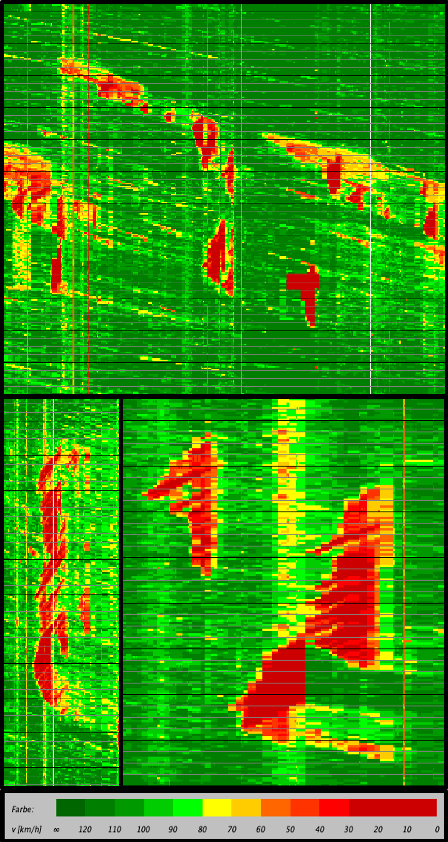
\includegraphics[scale=0.8]{./assets/SpeedMatrixPlot_mutiple}
	\caption{Speed matrix plots of processed FCD data, showing different jam clusters}
	\label{img:speedMatrixPlot_mutipleMixedClusters}
\end{figure}

The observer will clearly recognize the jams represented by the clusters of red and orange cells in the figure \ref{img:speedMatrixPlot_mutipleMixedClusters}, with the angled extends towards the right down edge, due to the vehicle trajectory through space and time. These cluster, also shown in the two lower pictures, which representing one or multiple jams can be densely packed or spotted into smaller clusters or, depending on the severity of a jam can be seen, by the cluster which contain more orange or yellow cells than red. 

From this visual clarity, the continuity of the data points and the precision on 3-minute intervals we can deviate that an algorithmic approach should also be able to detect such congestion events. This being said, the dataset does contain defects in the form of missing values for complete road sections, which can be easily ignored during processing. Another harder to detect and fixable defect type are visually obviously wrong speeds. Meaning sudden speed drops or jumps to block of identical speeds of an abnormal temporal and spatial extend. 

%Although originally an analysis of the whole year 2019 was planned, the provider was only able to deliver the FCD data for the first half in the timeframe of this thesis for processing and analysis. Due to that the evaluation time frame is restricted to the first half of the year 2019.

\section{BAYSIS}
\label{dataset_baysis}
\par The \acrfull{baysis} as describe in chapter \ref{dataset_baysis}, collects a wide range of different information types, which also contains accidents with the corresponding police reports. Accidents have a strong traffic influence on the Bavarian street network, with more than 400.000 being recorded in the year 2019 (StMi, 2020). The provided export contains all accidents of the year 2019 on the Bavarian highway network, which are 10262 records in number. Due to the limited availability of \acrshort{fcd} data and potential evaluation timeframe, only the accidents in the first half of the year 2019 are relevant. In these months 5140 accidents where recorded, which equivalents an expected 50\% of the total number of accidents on the highway network.
Each accident report includes a variety of specifications, which covers environmental indicators like weather or light situation, accident characteristics like accident type, collision object or cause, as well as information over the involved like nationality, age and gender. In total, one report contains 132 values, describing the accident, participant and environment. Because we do not want to form a stereotype of accident participant but rather find significant accident characteristics or environmental factors most of the descriptive values for the involved persons are not considered. Further we also have to neglect all values which cannot be converted in a numeric and nominal scale, due the used correlation methods. Variables, which don’t have any values are also neglected. From this curtailed pool of correlate able and analyze able characteristics we want to consider all parameters that have a logical significance with causes or effects of an accident.

A diverse distribution in the values would be also preferred, to reduce the risk of uncertain relation. Because the correlation of a non distributed variable, which for example has one values occupying a 95\% major share, is based on a sample set comprised of mostly the same samples, the interpretability for a correlation to other values but the major share is very limited (see \ref{correlation_uncertainty} for more detailed elaboration of this assumption).
\newline
\par To give an overview about what results can be expected on the basis of the provided dataset and which values are worth to be further evaluated, all plausible relevant parameters of the dataset will be illustrated and shortly discussed. All diagrams are also available as larger prints in the appendix \ref{appendix_baysis}. 

\begin{figure}[h]
	\centering
	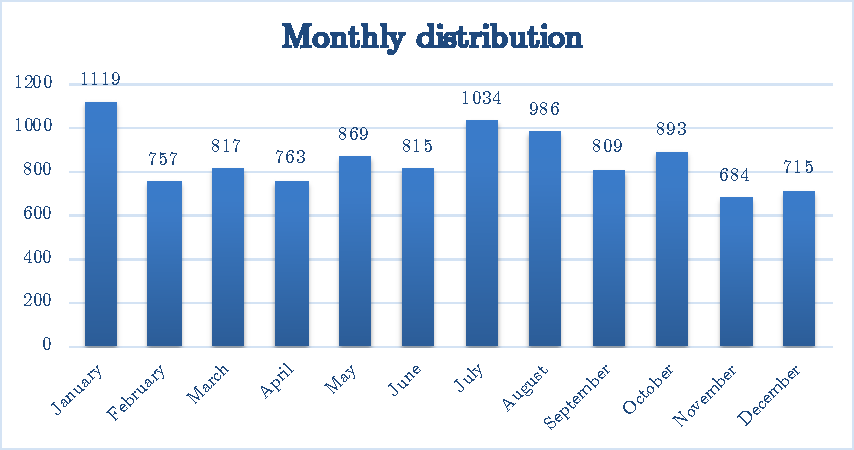
\includegraphics[scale=0.8]{./assets/baysis_dataset_monthly_absolute.pdf}
	\caption{Monthly distribution of absolute accident report counts}
	\label{img:baysis_monthlyDist_absolute}
\end{figure}

\begin{figure}[h]
	\centering
	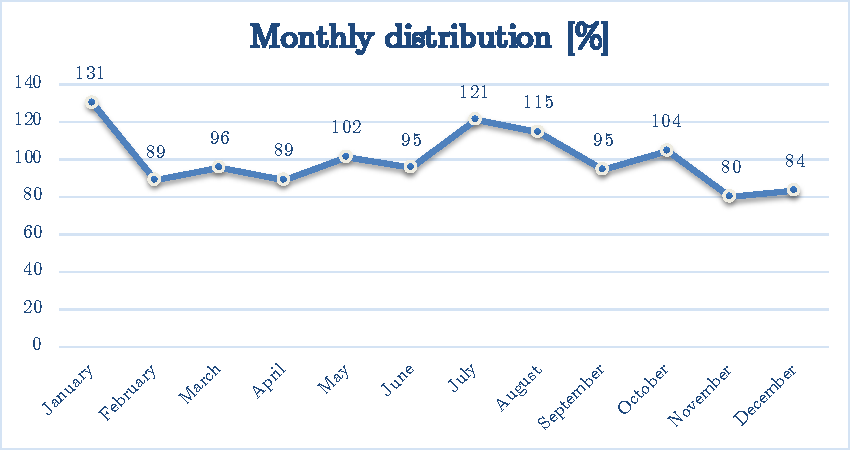
\includegraphics[scale=0.8]{./assets/baysis_dataset_monthly_percentage.pdf}
	\caption{Monthly distributions of accident report counts in percentages to mean}
	\label{img:baysis_monthlyDist_percentage}
\end{figure}

A look on the monthly distribution of accidents recorded by BAYSIS (shown in figure \ref{img:baysis_monthlyDist_absolute}) shows that there are no significant differences in number, besides of January. The monthly distribution expressed in percentages (see above in figure \ref{img:baysis_monthlyDist_percentage}) supports this deviation with a 31\% increase over the mean count of 857 accidents per month. This can be explained with the increased number of accidents due to ice and snow conditions, which reduces traction on roads and can lead to uncontrollable vehicle behavior in higher traveling speeds.

\begin{figure}[h]
	\centering
	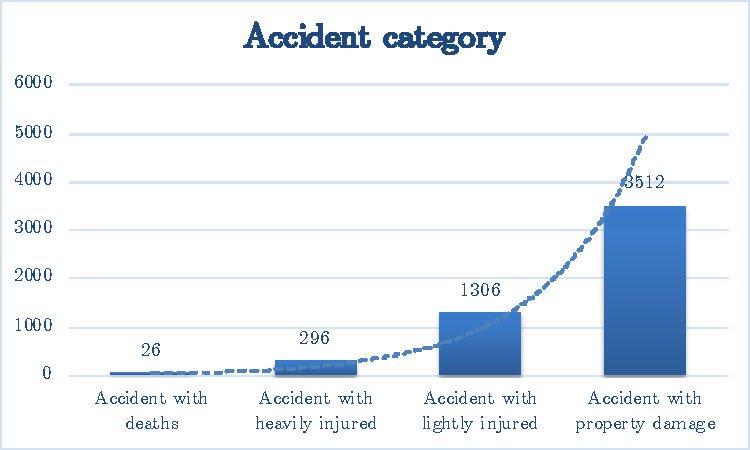
\includegraphics[scale=0.6]{./assets/baysis_dataset_Kat.pdf}
	\caption{Distribution of the accident category 'Kat'}
	\label{img:baysis_dataset_Kat}
\end{figure}

\paragraph{Kat}
The accident categories described by the variable shown in figure \ref{img:baysis_dataset_Kat}, presents a quite natural distribution. The categories range from just accident with damaged property to deathly accidents, with the number of deadly accidents having the lowest count. The distribution also fits the exponentially trend line, which allows the statement that statistical deadly accidents are exponentially unlikely. The variable consists of four values, which can be considered as ordered, and is therefore ordinal.

\begin{figure}[h]
	\centering
	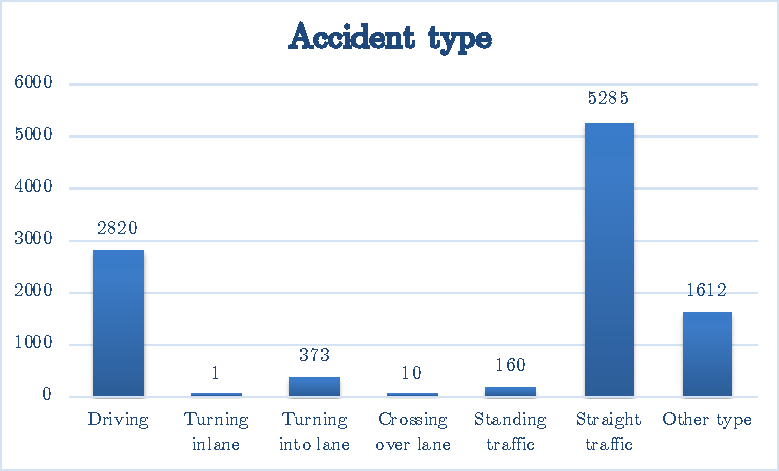
\includegraphics[scale=0.6]{./assets/baysis_dataset_Typ.pdf}
	\caption{Distribution of the accident type 'Typ'}
	\label{img:baysis_dataset_Typ}
\end{figure}

\paragraph{Typ}
The accident type variable (shown in figure \ref{img:baysis_dataset_Typ}) incorporates different kind of traffic movements, from straight and driving to turning movements. Beside of an 80\% share of accidents related to driving or straight driving situations, the parameter does not indicate any other features. The variable does not show any order and is therefore of nominal type.

\begin{figure}[H]
	\centering
	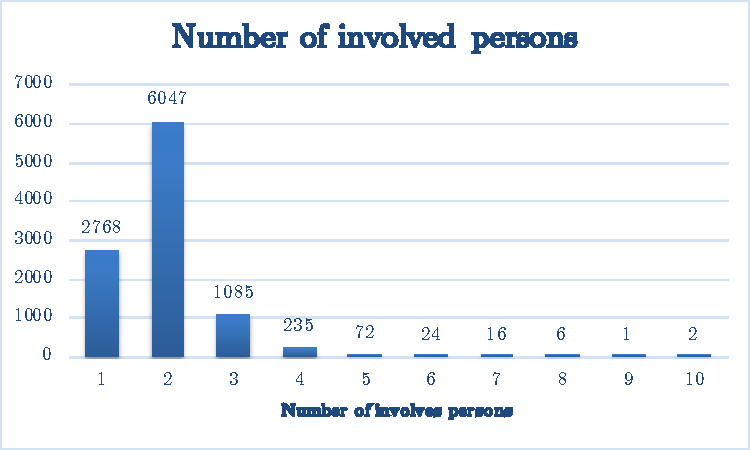
\includegraphics[scale=0.6]{./assets/baysis_dataset_Beteil.pdf}
	\caption{Distribution of the number of involves persons 'Beteil'}
	\label{img:baysis_dataset_Beteil}
\end{figure}

\paragraph{Beteil}
The distribution of the number of involved persons (shown in figure \ref{img:baysis_dataset_Beteil}) shows that more than 96\% of accidents have three or less involved persons. The major share of two involved persons makes up for 56\% and the second biggest of one involved person for 30\% of the total count. This also means the accidents with more than three involved persons are statistically insignificant. Because of the increasing oder of values, the variable is of ordinal type.

\begin{figure}[h]
	\centering
	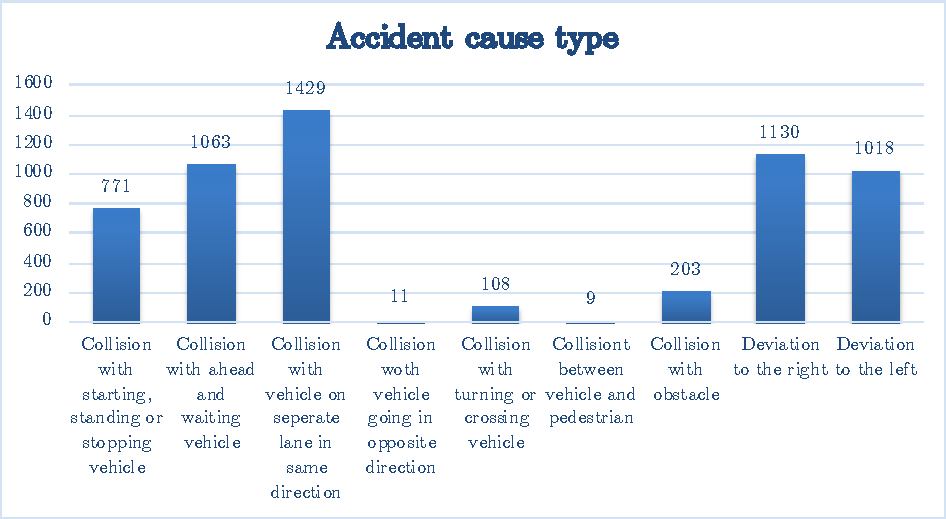
\includegraphics[scale=0.6]{./assets/baysis_dataset_UArt.pdf}
	\caption{Distribution of the accident cause type 'UArt'}
	\label{img:baysis_dataset_UArt}
\end{figure}

\paragraph{UArt}
The accident cause type, described by the two aggregated variables UArt1 and UArt2 (shown in figure \ref{img:baysis_dataset_UArt}), presents two major sets of causes. One being the accidents with waiting, stopping and starting vehicles in the same lane, which describe typical collision accidents during congested traffic. The other being the accidents in the next left or right lane, which describe common lane changing collisions. Accidents with cross traffic, pedestrians or opposite traffic are relatively uncommon. The variable does not show any order and is therefore of nominal type.

\begin{figure}[h]
	\centering
	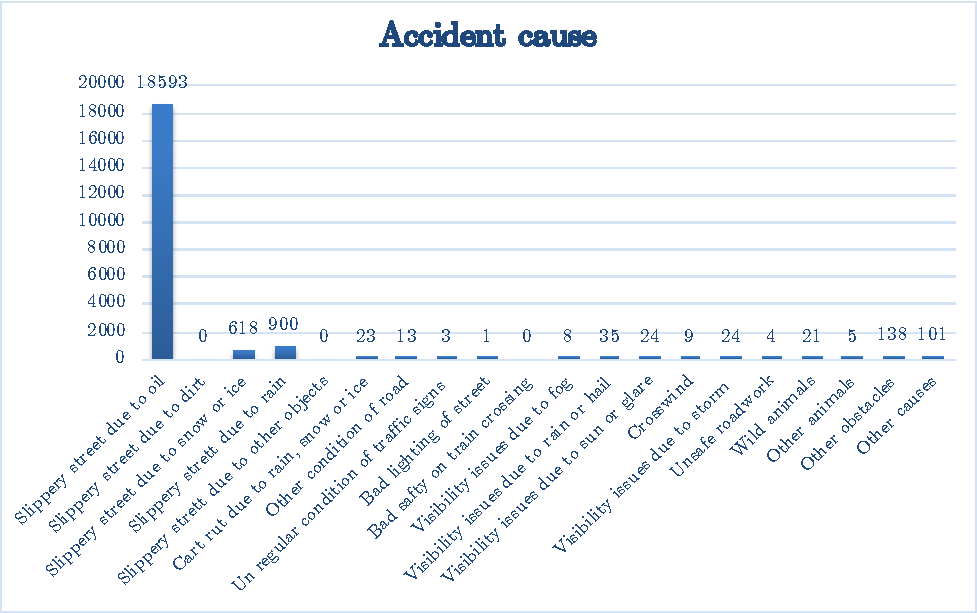
\includegraphics[scale=0.7]{./assets/baysis_dataset_AUrs.pdf}
	\caption{Distribution of the accident cause 'AUrs'}
	\label{img:baysis_dataset_AUrs}
\end{figure}

\paragraph{AUrs}
The summarized distribution of the parameters “AUrs1” and “AUrs2” (shown in figure \ref{img:baysis_dataset_AUrs}) does clearly that only the first category of “Slippery road condition due to oil” hold any significant share. Because of that any correlation to this parameter would not point to any usable statement and therefore can be neglected for the evaluation. The variable does not show any order and is therefore of nominal type.

\begin{figure}[]
	\centering
	\includegraphics[scale=0.6]{./assets/baysis_dataset_Aufhi.pdf}
	\caption{Distribution of obstacle collision 'AufHi'}
	\label{img:baysis_dataset_Aufhi}
\end{figure}

\paragraph{AufHi}
The obstacle collision distribution (shown in figure \ref{img:baysis_dataset_Aufhi}) reveals that in most collision accidents car hit the guardrails. The other categories are rather uncommon. With 1,5\% of accidents without any collision, it can be stated that in most cases a collision is part of an accident. The counts of the remaining categories are insignificant. The variable does not show any order and is therefore of nominal type.

\begin{figure}[h]
	\centering
	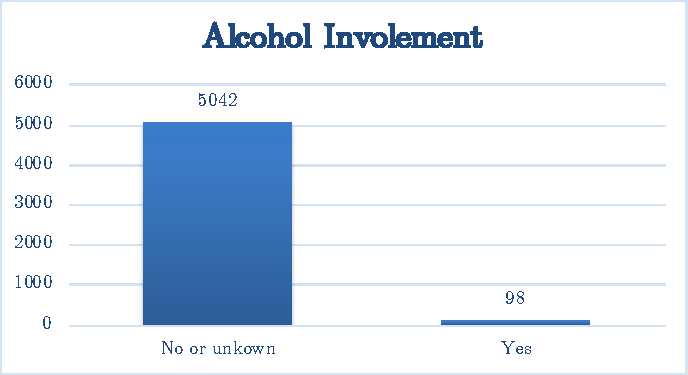
\includegraphics[scale=0.6]{./assets/baysis_dataset_Alkoh.pdf}
	\caption{Distribution of the alcohol Involvement 'Alkoh'}
	\label{img:baysis_dataset_Alkoh}
\end{figure}

\paragraph{Alkoh}
The Alcohol involvement indication parameter (shown in figure \ref{img:baysis_dataset_Alkoh}) shows that 1,9\% of accidents have one or more involved persons with measurable alcohol amounts in the blood connected with it. The respective 98 reports with 
	%TODO variabel type

\begin{figure}[h]
	\centering
	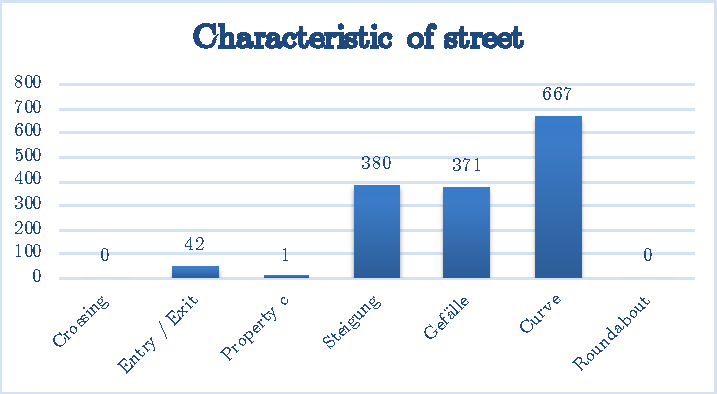
\includegraphics[scale=0.6]{./assets/baysis_dataset_Char.pdf}
	\caption{Distribution of the street characteristic 'Char'}
	\label{img:baysis_dataset_Char}
\end{figure}

\paragraph{Char}
The variable distribution shown in figure \ref{img:baysis_dataset_Char} describes the characteristic of the street where the accident happened. Since we are only considering highway, the type of “crossing” is expected to be zero. 
	%TODO variabel type

\begin{figure}[h]
	\centering
	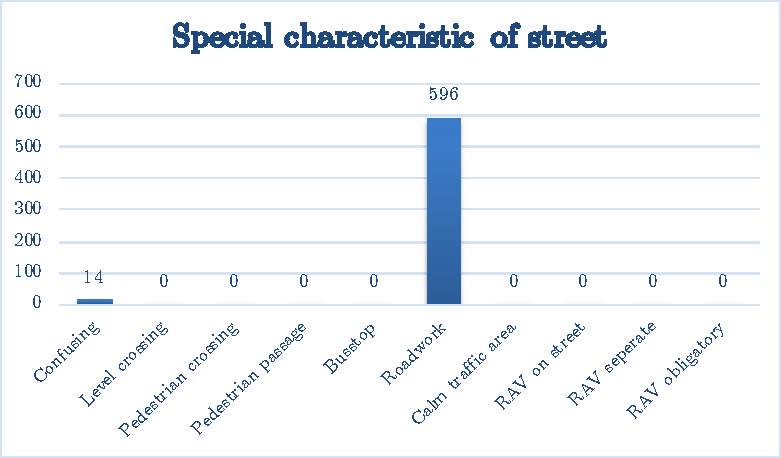
\includegraphics[scale=0.6]{./assets/baysis_dataset_Bes.pdf}
	\caption{Distribution of the special street characteristic}
	\label{img:baysis_dataset_Bes}
\end{figure}

\paragraph{Bes}
The aggregated distribution of the variables Bes1, Bes2 and Bes3, which further defines the street characteristic mentioned above.
	%TODO variabel type 

\begin{figure}[h]
	\centering
	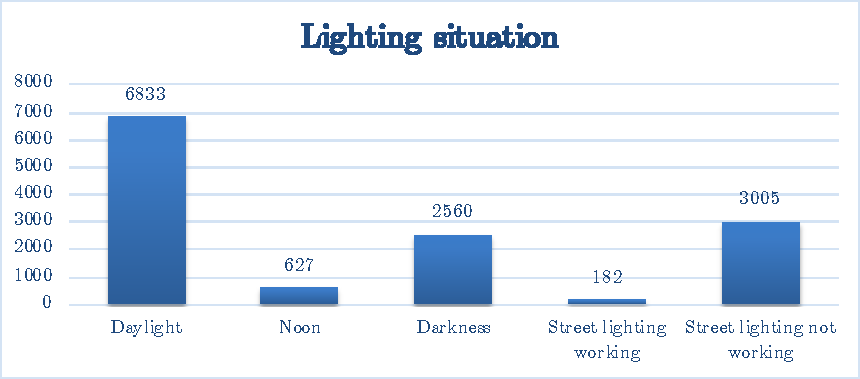
\includegraphics[scale=0.6]{./assets/baysis_dataset_Lich.pdf}
	\caption{Distribution of the lighting situation}
	\label{img:baysis_dataset_Lich}
\end{figure}

\paragraph{Lich}
Dolorem Ipsum. Dolorem Ipsum. Dolorem Ipsum. Dolorem Ipsum.
Dolorem Ipsum. Dolorem Ipsum. Dolorem Ipsum. Dolorem Ipsum.
Dolorem Ipsum. Dolorem Ipsum. Dolorem Ipsum. Dolorem Ipsum.
	%TODO variabel type

\paragraph{Zust}
\begin{figure}[h]
	\centering
	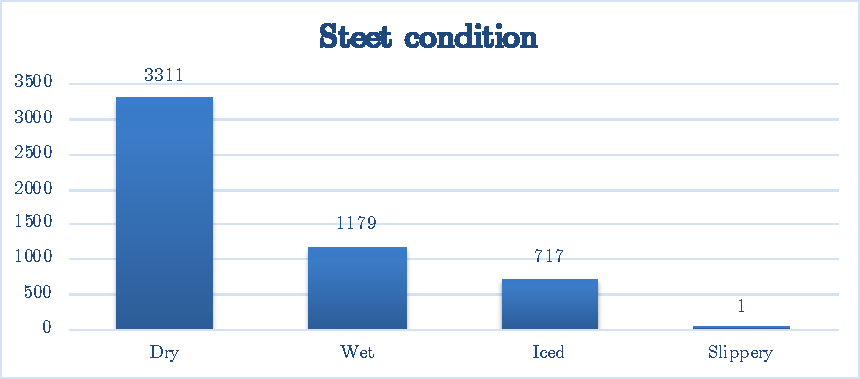
\includegraphics[scale=0.6]{./assets/baysis_dataset_Zust}
	\caption{Distribution of the street condition}
	\label{img:baysis_dataset_Zust}
\end{figure}

Dolorem Ipsum. Dolorem Ipsum. Dolorem Ipsum. Dolorem Ipsum.
Dolorem Ipsum. Dolorem Ipsum. Dolorem Ipsum. Dolorem Ipsum.
Dolorem Ipsum. Dolorem Ipsum. Dolorem Ipsum. Dolorem Ipsum.
	%TODO variabel type

\paragraph{Fstf}
\begin{figure}[H]
	\centering
	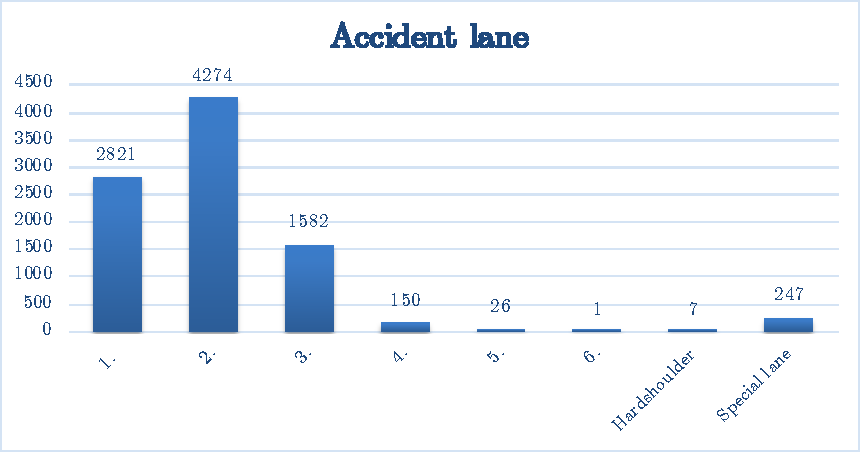
\includegraphics[scale=0.6]{./assets/baysis_dataset_Fstf.pdf}
	\caption{Distribution of the number of closed lanes}
	\label{img:baysis_dataset_Fstf}
\end{figure}


\begin{figure}[H]
	\centering
	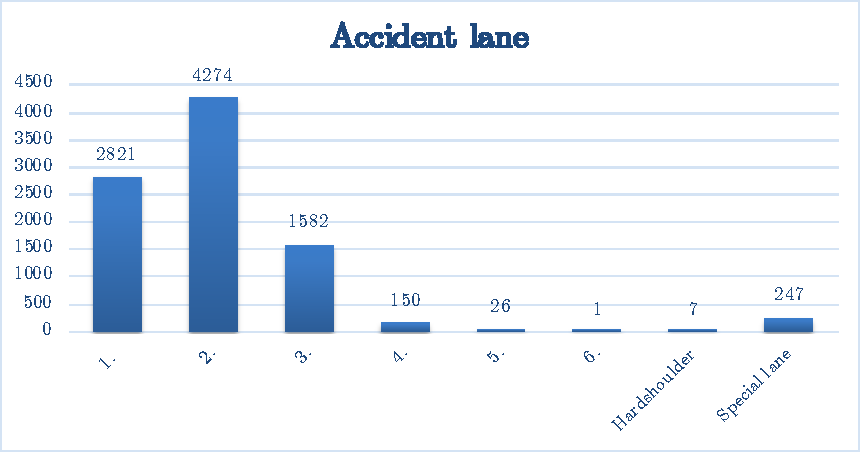
\includegraphics[scale=0.6]{./assets/baysis_dataset_Fstf.pdf}
	\caption{Distribution of the number of closed lanes}
	\label{img:baysis_dataset_Fstf}
\end{figure}

\paragraph{WoTag}
The variable of WoTag relates to the day of week, when the accident happened. 

\paragraph{FeiTag}
Form the total of ??, 157 accidents to place during a public holiday.
	
\begin{table}[ht]
	\centering
	\begin{tabular}{c|c|c}
		\textbf{Variable} 	& \textbf{Group} 	& \textbf{Type} 		\\
		\\[-1em]
		\hline
		\\[-1em]
		Kat  		& categorical 	& ordinal 	\\
		\\[-1em]
		\hline
		\\[-1em]
		Typ 		& categorical 	& nominal	\\
		\hline
		\\[-1em]
		Beteil 		& categorical 	& ordinal	\\
		\hline
		\\[-1em]
		UArt 		& categorical 	& nominal	\\
		\hline
		\\[-1em]
		AUrs 		& categorical 	& nominal	\\
		\hline
		\\[-1em]
		AufHi 		& categorical 	& nominal	\\
		\hline
		\\[-1em]
		Alkoh 		& categorical 	& dichotomous	\\
		\hline
		\\[-1em]
		Char 		& categorical 	& nominal	\\
		\hline
		\\[-1em]
		Bes 		& categorical 	& nominal	\\
		\hline
		\\[-1em]
		Lich 		& categorical 	& nominal	\\
		\hline
		\\[-1em]
		Zust 		& categorical 	& nominal	\\
		\hline
		\\[-1em]
		Fstf 		& categorical 	& nominal	\\
		\hline
		\\[-1em]
		Strst 		& categorical 	& nominal	\\
		\hline
		\\[-1em]
		WoTag 		& categorical 	& nominal	\\
		\hline
		\\[-1em]
		FeiTag 		& categorical 	& dichotomous	\\
	\end{tabular}
	\caption{\label{tab:table-name}Variable types of \acrshort{baysis} dataset}
\end{table}



The figure \ref{img:correlation_matrix_dataset} shows the correlation coefficient of each mentioned accident characteristic 

\begin{figure}[h]
	\centering
	\includegraphics[scale=0.2]{../Analyse/data/BAYSIS/dataset/correlation_matrix.png}
	\caption{Correlation matrix for BAYSIS dataset, calculated with \ref{definition_correlation} and \ref{definition_correlation_script} (for larger print see Appendix ??)}
	\label{img:correlation_matrix_dataset}
\end{figure}

For further use, we do not want to work with the \acrshort{csv} file format in which the dataset was provided. Because the designed analyzation and evaluation tool, utilizes a PostgreSQL database for its data storage we need to process and convert the accident reports into data entities. Also, the data entities for each accident need to be uniform and comparable with our street network and other entities like roadworks, which makes it necessary to process and map the accidents onto our street network. After the processing and import into the database, 7971 records end up being converted and persisted, which equivalent to 76,6\% of the provided number of accidents for these months or 25,8\% of all accidents. This 23,5\% of data loss is due to the conversion of location or position data from the BAYSIS dataset to our street net-work. In this process we try to find a corresponding street network location to the legacy location of the BAYSIS dataset. If we are not able to locate the position of the BYSIS dataset on our street network we discard the record, because we can’t work with it downstream. 

\section{ArbIS}
\label{dataset_arbis}

The \acrfull{arbis}, as described in chapter \ref{dataset_arbis}, is a collection service of all roadworks or maintenance planned, ongoing or finished on the Bavarian street network. With the 4500 long term and more than 40.000 short term building sites on German highways per year \cite{LAPID2018,Stmi2020}, road construction make up for the majority of traffic obstructions in the summer months, when during the colder month, in which many kinds of construction projects are not possible, snow clearings or long-term constructions are the issue. That also means that the number and type of roadworks heavy varies during the course of a year (StmB, 2020). Because the limited evaluation time only the road-works till April are relevant, which arguably are the colder months and therefor contain mostly snow clearings and long-term construction obstructions, this could potentially bias the results due to the missing, but equality important short-term construction roadworks.
\par The dataset for 2019 contains close to 650.000 datapoints, which each describe the temporal and spatial extend, road name and number of closed lanes of a roadwork fragment. This fragmentation of events makes is rather hard to statically analyze this dataset since each roadwork is spitted into any number of fragments in now recognizable pattern and are only linked by a roadwork identifier. Therefore the analysis of the dataset in this section is rather basic.
\par After the selection of the relevant incidents from the first half year of 2019, 302.799 datapoints remain, which will be converted and imported like the \acrshort{baysis} data, described in chapter \ref{dataset_baysis}. This processing and aggregation of fragments produce 129.874 roadwork events in the database, which monthly distribution is shown in figure \ref{img:arbis_dataset_monthly_absolute}


\begin{figure}[h]
	\centering
	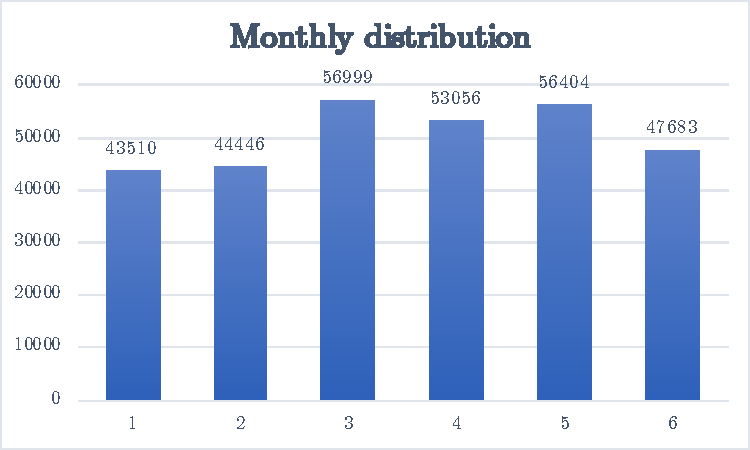
\includegraphics[scale=0.6]{./assets/arbis_dataset_monthly_absolute}
	\caption{Monthly distribution of absolute roadwork data entry counts}
	\label{img:arbis_dataset_monthly_absolute}
\end{figure}


\begin{figure}[h]
	\centering
	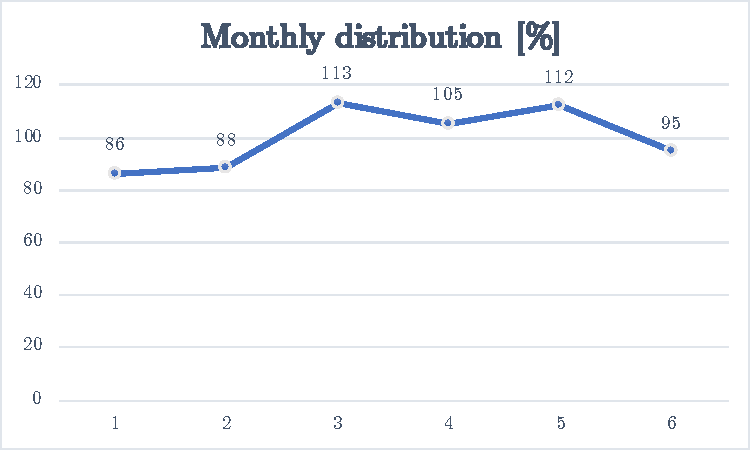
\includegraphics[scale=0.6]{./assets/arbis_dataset_monthly_percentage}
	\caption{Monthly distributions of roadwork data entry counts in percentages to mean}
	\label{img:arbis_dataset_monthly_percentage}
\end{figure}




\chapter{Methodology}
The central goal of the thesis it to determine if jams characteristics, detected in \acrshort{fcd} data and incident characteristics from accidents (\acrshort{baysis}) and roadworks (\acrshort{arbis}) do correlate with each other. Therefore, the main research question to be answered stands as followed:

\begin{center}
	\textit{Is there a correlation between FCD congestion and incident characteristics?}
\end{center}

\bigskip

\par Assuming that there is a correlation of congestion and incident characteristics, the second and more interpretable question would arise.

\begin{center}
	\textit{Can the correlation of FCD congestion and incident characteristics predict the possibilities of a consecutive events?}
\end{center}

\bigskip

To answer these research questions, there are a series of steps involved, from identifying congestion event in the FCD data and finding adjacent incident events to comprising a unified dataset and evaluating the results.

\bigskip

The \acrshort{fcd} data, as described in \ref{dataset_fcd}, is a nearly continuous series of datapoint which represents the mean absolute and relative speed of the street section at each 3-minute interval on a road section. In \ref{dataset_fcd} we determined that thought a manual visual analysis jams can be easily identified. This manual identification needs to be automated because of the amount of data representing a complete year and all Bavarian highways. Such an automated process needs to be able to find congestion events and defined dimensions, shape as well as characteristic values. For the correlation analysis of jams to incidents, the detection of adjacent incident is needed.

The \gls{evaltool} from the \gls{congstats} service, the project which inspired this thesis, was developed for exactly this purpose and will be expanded to fit the required specification.

\section{Detection Algorithm}
First step is the detection of congestion events. The definition in \ref{definition_congestion} states that a congestion is a dense, timely and spatial accumulation of jammed cells, also describable as cluster of jammed cells. Therefore a clustering algorithm would be suitable to identify congestion events.

For the classification of the congestion events into different types, by theirs spatial and timely extends a shaping algorithm is needed. It is supposed to convert the accumulation of cells into a simple describable shape, which can be put into groups.

\subsection{Clustering}
The term clustering is the short form of a data mining technique also called numerical taxonomy or cluster analysis with the goal of finding data structures or associations. For this purpose a multitude of algorithms where developed over time, varying in they strategies, methods and performance \cite{Busch2004}. E.g. k-means or k-metoid (point distance), affinity propagation (graph distance), mean-shift (point distance), DBSCAN (nearest point distance), gaussian mixtures (mahalanobis distance to centers), spectral clustering (graph distance) \cite{Chauhan2020}.

% https://texample.net/tikz/examples/probability-tree/
% https://webis.de/downloads/theses/papers/busch_2005.pdf 1.6
%\begin{tikzpicture}[grow=right, sloped]
%\node[bag] {Cluster Algorithms}
%    child {
%        node[bag] {hierarchic}        
%             child {
%                node[end, label=right:
%                    {single-linkage, group-average}] {}                
%                edge from parent
%            }         
%            edge from parent 
%    }
%    child {
%        node[bag] {iterative}        
%            child {
%                node[end, label=right:
%                    {k-means, k-metoid, Kerninghan-Lin}] {}                
%                edge from parent
%            }         
%            edge from parent 
%    }
%    child {
%        node[bag] {density-based}        
%            child {
%                node[end, label=right:
%                    {DBSCAN, MajorClust}] {}                
%             	edge from parent
%            }
%            edge from parent
%    }
%	child {
%        node[bag] {meta-search}        
%                 child {
%                node[end, label=right:
%                    {genetic algorithms}] {}
%                edge from parent
%            }            
%            edge from parent
%    }
%    child {
%        node[bag] {statistical}        
%        child {
%                node[end, label=right:
%                    {gaussian mixtures}] {}
%                edge from parent
%            }
%            edge from parent         
%    };
%\end{tikzpicture}

\bigskip

\begin{figure}[h]
	\centering
	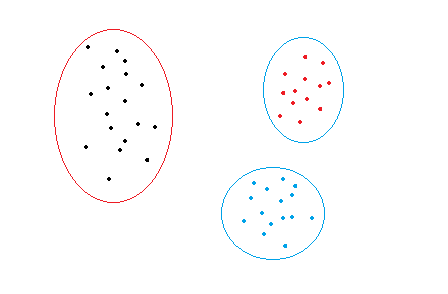
\includegraphics[scale=0.5]{./assets/cluster_seperate.png}
	\caption{Example clustered by k-means algorithm \cite{Yildirim2020}}
	\label{cluster_kmeans}
\end{figure}

To illustrate which problems can occur when using cluster algorithms and to defined the major features to find the most suitable one, the k-means is used as base comparison or starting point. The figure \ref{cluster_kmeans} shows three differently colored groups of points, which are clustered into three clusters, represented by the circles around the groups. It demonstrates the general principle of clustering and was done by the common k-means algorithm with the $a$ $priori$ parameter of three clusters. 

\begin{figure}[h]
	\centering
	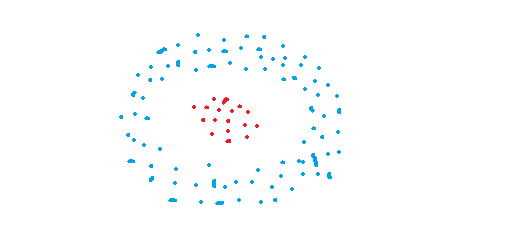
\includegraphics[scale=0.4]{./assets/cluster_1.png}
	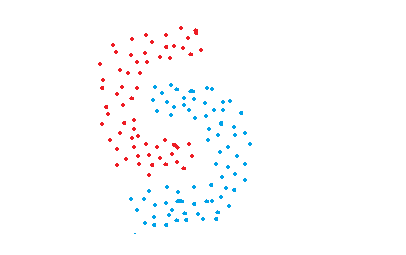
\includegraphics[scale=0.4]{./assets/cluster_2.png}
	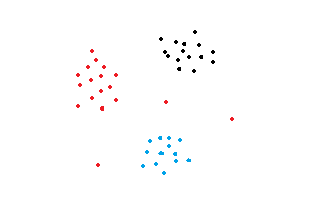
\includegraphics[scale=0.4]{./assets/cluster_3.png}
	\caption{Example clustered by density-based algorithm \cite{Yildirim2020}}
	\label{cluster_dbscan}
\end{figure}

This works well as long as the groups don't overlay, intersect or have arbitrary shapes like in the figures \ref{cluster_dbscan}. When this is the case, the k-mean may cluster loosely related point together, which actually are more strongly related to other points, because it considers every point as possible neighbor. Since jams in FCD data can overlay and have any number of shape, as suitable algorithms need to be able to handle such data.

Another issue with this method is the vastly increasing runtime when processing larger amounts of data. The objective function (shown in formula \ref{formula_kmeans}) of the k-mean algorithm states that $n$ distances are calculated for $k$ points \cite{Santhanam2010}. With this equation and the assumption that every distance for every point will be calculated and therefore $k=n$, the Big $\Theta$ notation, commonly known as Big $O$, describing the scaleable time complexity of an algorithm, is $O(n \cdot K \cdot I \cdot d)$ ($n$ = number of points, $K$ = number of clusters, $I$ = number of iterations, $d$ = number of attributes) \cite{Dalatu2016}. It is commonly simplified in literature to $O(n^2)$, a quadratic complexity \cite{Pakhira2014}. The assumption also entails that in a worst case scenario $n^n$ calculations have to me computed over all iterations.

\begin{equation}
\label{formula_kmeans}
	J =  \sum_{j=1}^k{\sum_{i=1}^n{\abs{x_i^j-c_j}}}
\end{equation}

\bigskip

A Big $O$ notation of $O(n^2)$ can generally be described as inefficient, but if we would apply the worst case scenario as an example on the data of the highway A3 and a timeframe of 24 hours, which contains 836.752 data points, the runtime issue becomes quite obvious. As the equation \ref{equation_kmeans_nn} show, the total number of calculation is so astronomical high, that it would take days to run this cluster. \cite{Busch2004}

\begin{equation}
\label{equation_kmeans_nn}
	 = 836752^{836752} = 4.8234... \cdot 10^{4955744}
\end{equation}

\bigskip

Entering density-based methods, which are better suited to identify distinctive, arbitrary clusters in in large datasets, by looking for a contiguous region of high point density, separated from others by contiguous regions of low point density \cite{Chauhan2020}. 

\subsubsection{Algorithm}

The DBSCAN algorithm, standing for \textbf{d}ensity-\textbf{b}ased \textbf{s}patial \textbf{c}lustering of \textbf{a}pplications with \textbf{n}oise, is able to find arbitrary shaped cluster and clusters by considering the spatial density, which also represents noise  \cite{Yildirim2020,Chauhan2020}. The basic idea of this algorithm is to form cluster of points, which are close too \textbf{many} other points of the cluster. For this strategy two thresholds parameters are needed. The first being the minimal size of a cluster, referred to as $minPts$, which defines the minimum number of points of a cluster to be considered as dense. And secondly the maximum distance threshold between cluster points, $eps$ ($\varepsilon$). \cite{Yildirim2020,Chauhan2020} 

With these thresholds data points can be classified as core point, border point or outliner.

\begin{itemize}
	\item \textbf{Core points} have at least the $minPts$ number of points around them within the radius $eps$, including itself.
    \item \textbf{Border points} 
 	\item \textbf{Outliers} 
\end{itemize}

Finds core samples of high density and expands clusters from them.



DBSCAN with expansion of removing wrong and small, and combining small and near

%https://www.kde.cs.uni-kassel.de/wp-content/uploads/ws/LLWA03/fgml/final/Kirchner.pdf
%https://www.researchgate.net/publication/322729622_Characterizing_Diffusion_Dynamics_of_Disease_Clustering_A_Modified_Space-Time_DBSCAN_MST-DBSCAN_Algorithm
%https://www.nature.com/articles/s41598-017-12852-z
%http://citeseerx.ist.psu.edu/viewdoc/download?doi=10.1.1.63.1629&rep=rep1&type=pdf
%http://cucis.eecs.northwestern.edu/publications/pdf/HAL18.pdf

\subsubsection{Distance Measuring}

\subsubsection{Performance Tuning}

\subsection{Shaping}

Convex Hull
%https://www.diva-portal.org/smash/get/diva2:931027/FULLTEXT02

\section{Matching Algorithm}
We now have a list of jams, found on the matching incidents with spatial and timely adjacent congestions
See CONGSTATS Matching Algorithm (own implementation)

\section{Data Processsing}
\label{methodology_data_generation}
Until now all data is in the CONGSTATS system. Export to analyzable format is necessary.
Which values where converted into numeric values and why and …

\section{Correlation Processing}
\label{definition_correlation_script}

Explain python script for correlation analysis

\cite{Potvin2020}


\chapter{Analysis}

Analysis of the resulting separate datasets of congestion and incidents. What characteristic and key indicators are prominent?
\section{Features}
What find of values, features and so on, does the dataset contain?
\section{Time and space dimension}
What time frame does the dataset cover and over what spatial area.
\section{Containing information}
What kind of information does the dataset contain?
\section{Integrity and short comings}
What kind of information does the dataset contain?

\chapter{Interpretation}

\section{Assocations}

\section{Predictions}
Is the correlation strong enough to use it for predicting congestions and accidents?

\subsection{Prediction of Accidents}

\subsection{Prediction of Congestions}

\chapter{Implementation}

\section{Requirements}

\section{Data Aviability}

\chapter{Conclusion}

\section{Answer of research question}

\section{Usability of results and interpretation}

\section{Future development and possible improvements} 

expand dbscan to 3d from 2d to include cell speed

%\subsubsection{... Test}
%\paragraph{... Test}
%\subparagraph{... Test}

\addcontentsline{toc}{chapter}{Bibliography}
\bibliographystyle{apalike}
\bibliography{../Literatur/library}{}

\addcontentsline{toc}{chapter}{List of Figures}
\listoffigures

\addcontentsline{toc}{chapter}{List of Tables}
\listoftables

\printglossary[title=List of Acronyms, type=\acronymtype]

\printglossary[title=List of Terms]

\begin{appendices}

\chapter{BAYSIS Dataset Figures}
\label{appendix_baysis}

\tocless\section{}
\label{appendix_baysis_dataset_corr_cramers}
\begin{figure}[H]
	\centering
	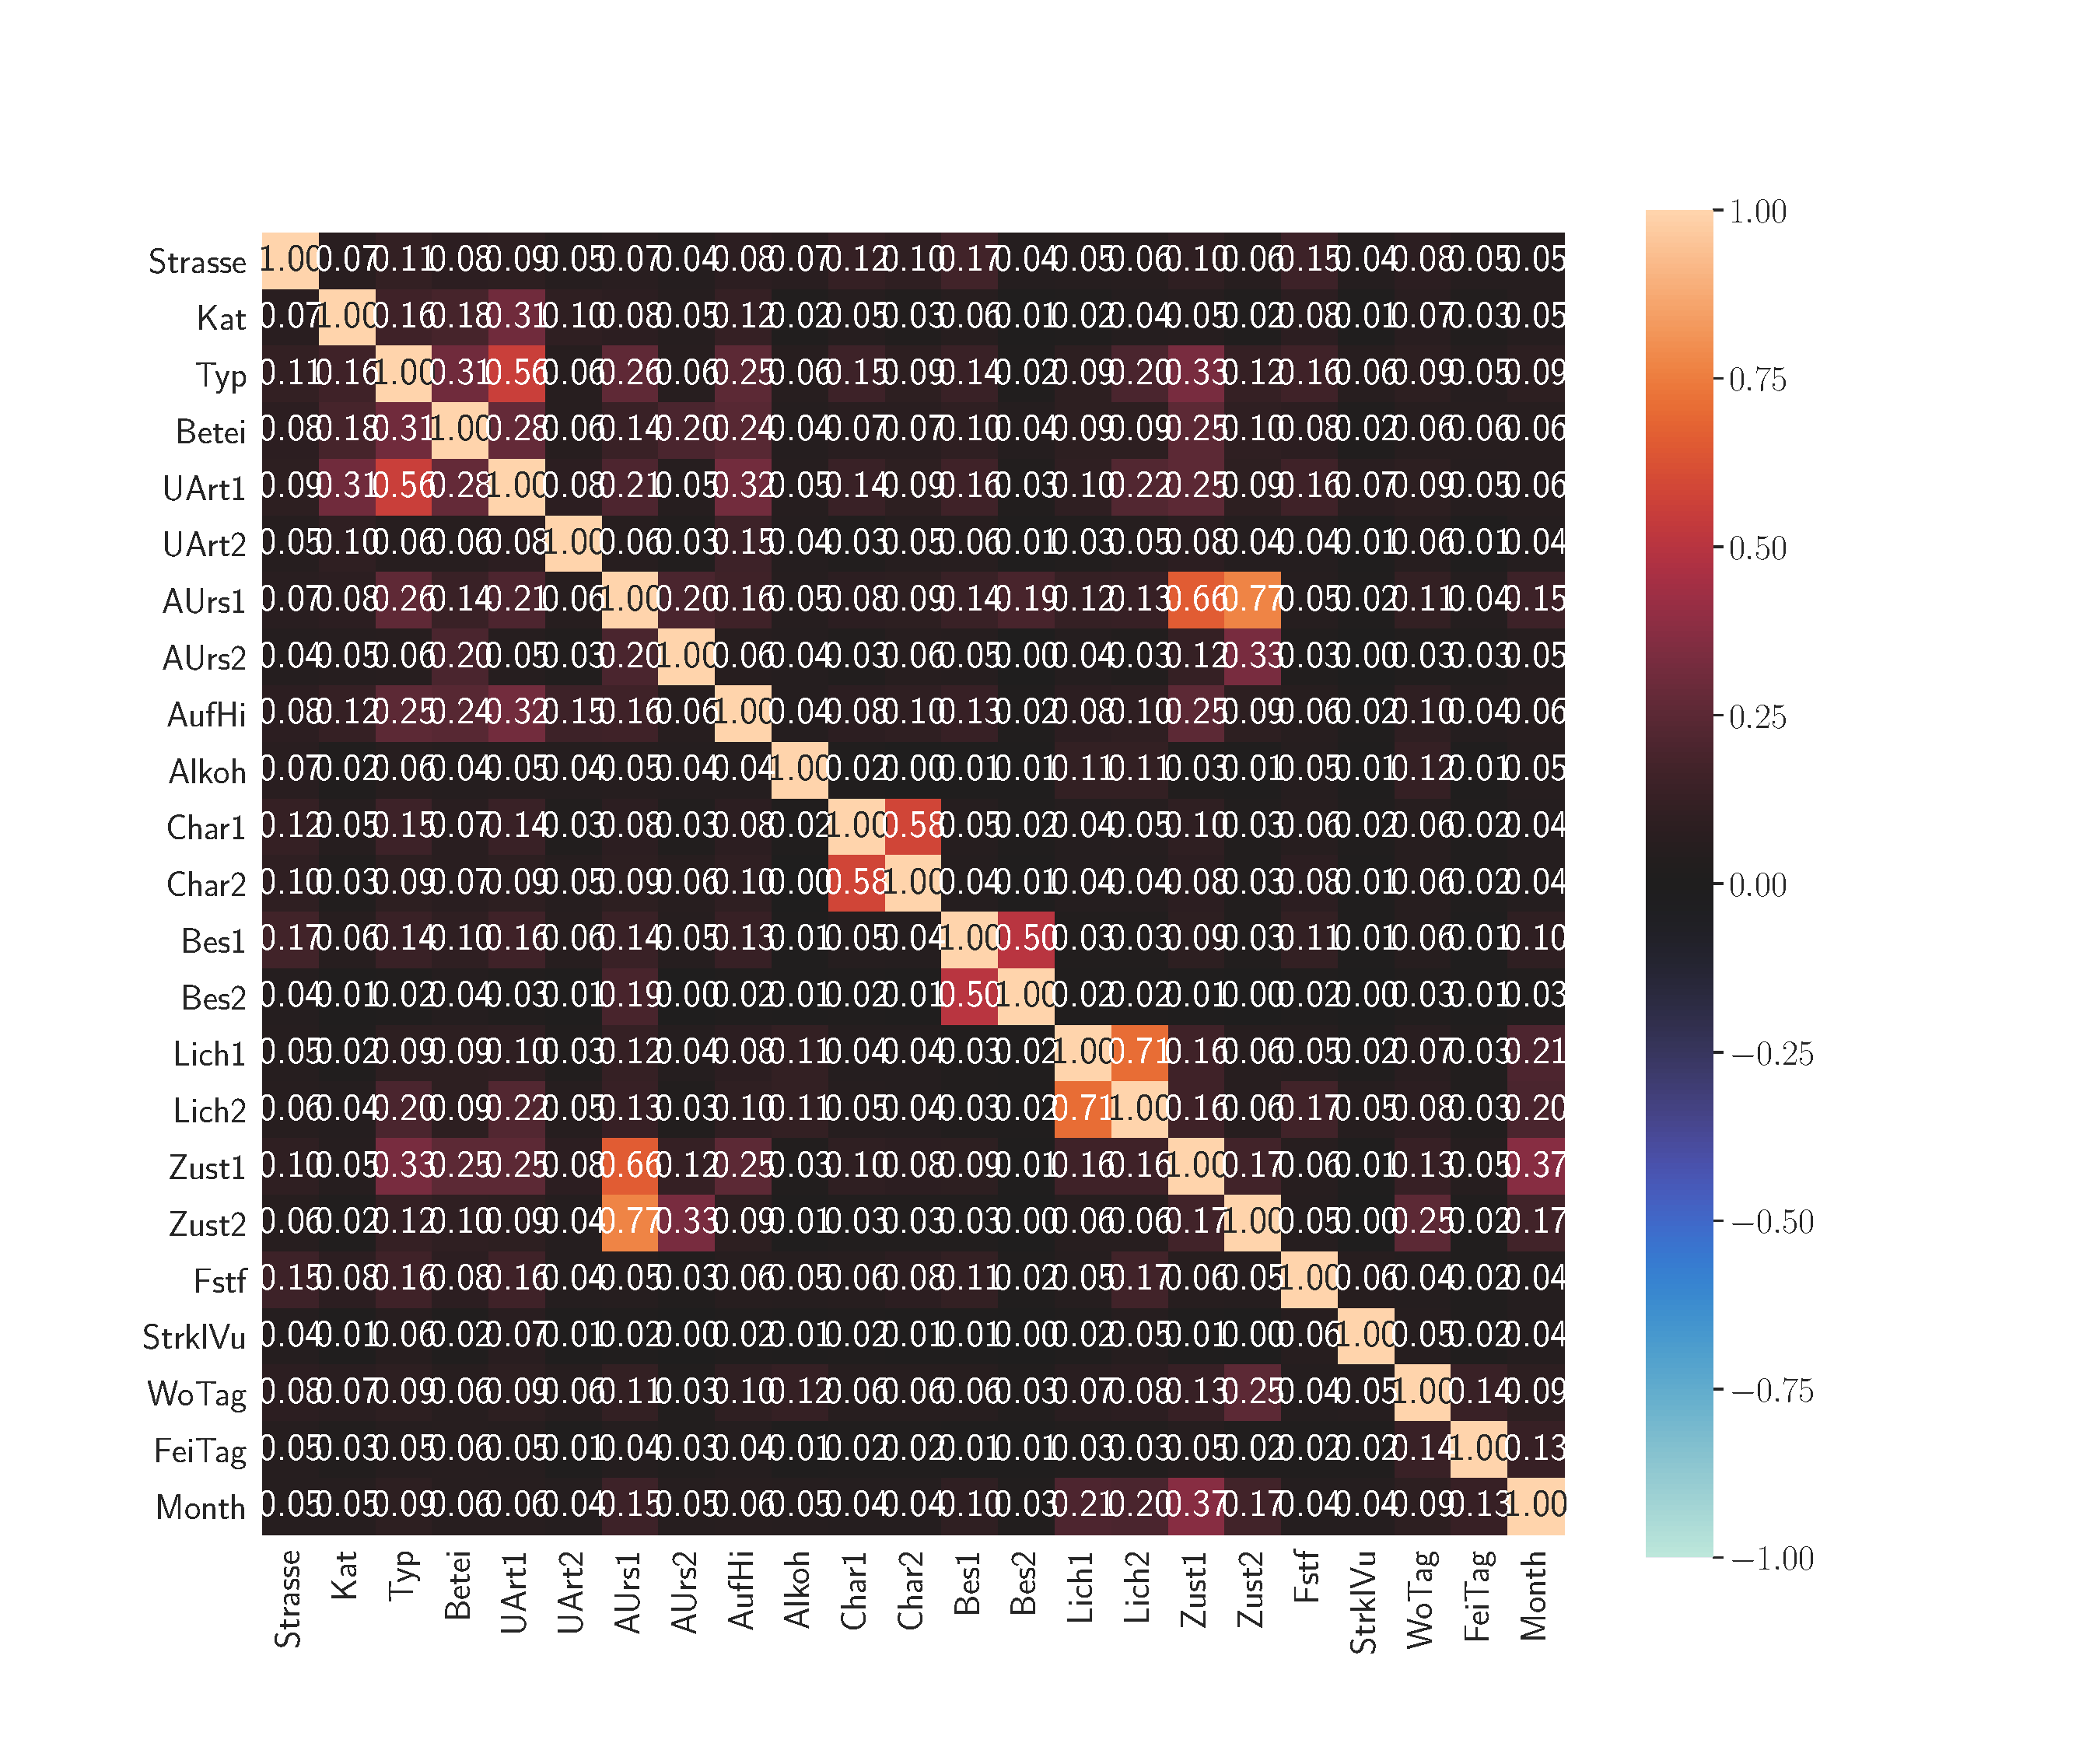
\includegraphics[scale=0.3]{../Analyse/data/BAYSIS/dataset/plots/baysis_dataset_corr_cramers}
	\caption{Correlation matrix for BAYSIS dataset, calculated with \ref{definition_correlation} and \ref{definition_correlation_script}}
	\label{img:appendix_correlation_matrix_dataset}
\end{figure}

\tocless\section{}
\label{appendix_baysis_dataset_corr_theils}
\begin{figure}[H]
	\centering
	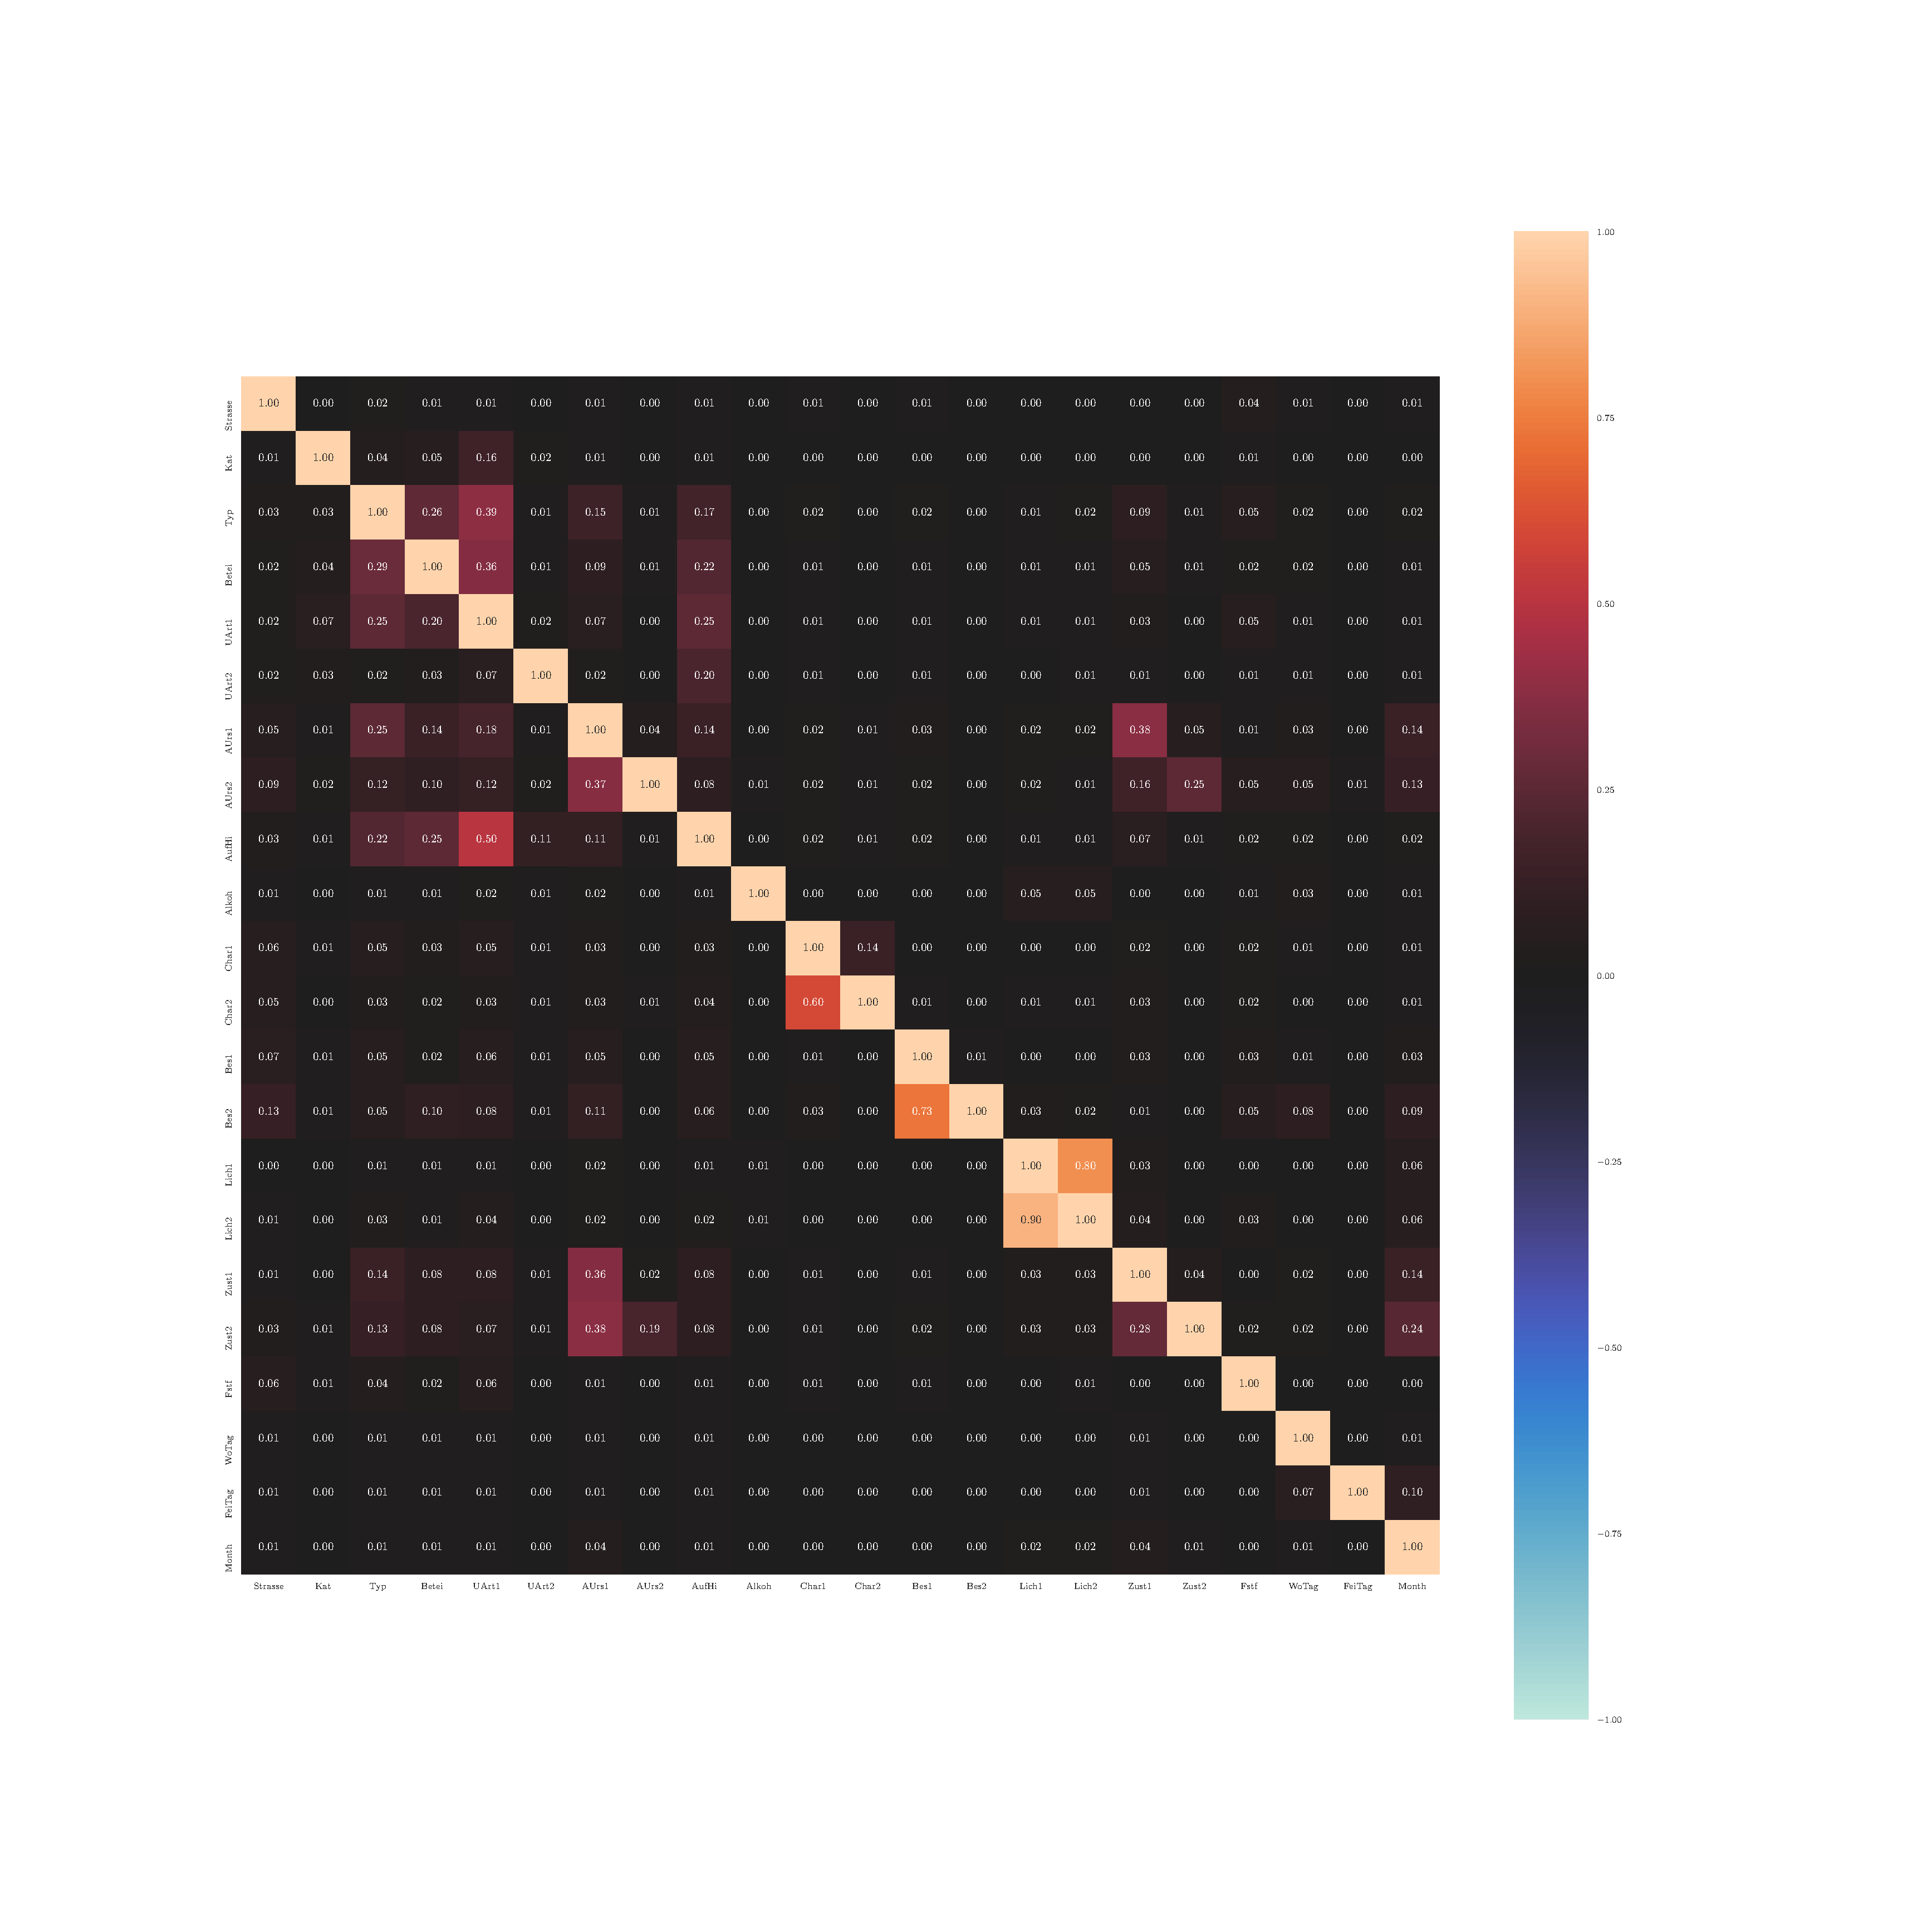
\includegraphics[scale=0.3]{../Analyse/data/BAYSIS/dataset/plots/baysis_dataset_corr_theils}
	\caption{Correlation matrix for BAYSIS dataset, calculated with \ref{definition_correlation} and \ref{definition_correlation_script}}
	\label{img:appendix_correlation_matrix_dataset}
\end{figure}


\chapter{ArbIS Dataset Figures}
\tocless\section{Figure Name}
\label{appendix_TODO}
%TODO add all BAYSIS figures as large print

\chapter{Source Code}

\tocless\section{CongstatsClusterAlgorithm}
\label{appendix_TODO}

\newgeometry{left=2cm,top=0.5cm,bottom=0.5cm}
\begingroup
%    \fontsize{4pt}{8pt}\selectfont
%		\lstinputlisting[language=java]{../Code/congestion/clustering/CongstatsClusterAlgorithm.java}
\endgroup
\restoregeometry

\end{appendices}

\pagebreak
\addcontentsline{toc}{chapter}{Declaration of independence}
\chapter*{Declaration of independence}
Erklärung zur Master’s Thesis
\newline \\
Ich versichere hiermit, die vorliegende Arbeit selbständig verfasst und keine anderen Quellen als die angegebenen Quellen und Hilfsmittel benutzt zu haben. Die Arbeit wurde noch nicht anderweitig für Prüfungszwecke vorgelegt. 
\newline \\ \\ \\
München, 15.12.2020: \hrulefill \newline
\hspace*{0mm}\phantom{München, 11.12.2020: } B. Sc. Jakob Erpf

\end{document}
